\chapter{Flexible Interactive Retrieval System and Best Practices for Visual Retrieval}
\label{chap-first}
\begin{ChapAbstract}
In this chapter, we describe our retrieval system called FIRST in details. We provide an overview of the system in Section \ref{sec:FIRST_overview} and discuss our system design in Section \ref{sec:first_system_design}. Section \ref{sec:first_front_end_design} concerns the user interfaces and interactions, while Section \ref{sec:first_back_end_design} focuses on the AI-related components that assist the user during the retrieval process. Finally, in the last three sections, we introduce more details about the Lifelog Search Challenge 2022 and Visual Browser Showdown 2022, the evaluation metrics used in these challenges and the result of our interactive retrieval system on each challenge.
\end{ChapAbstract}
\section{Overview}
\label{sec:FIRST_overview}

Our application is designed as a web application consisting of four main parts: the front-end, back-end, AI model server, and databases (Figure \ref{fig:Retrieval_architecture}). We choose to build a web application instead of a native one because it better supports the separation of each component over the network and hence, easier development and deployment. The components communicate via APIs over HTTP/HTTPS protocols, therefore they can be either on the same machine, on a different machine, or even on a cluster of multiple nodes. Although this greatly pile up the tech stack and hence make it much more challenging, it shows our seriousness in developing a system that is similar to real-world systems, where it comprises of many pieces and each part requires an expert in that field (e.g., database, front-end developer, etc.) to develop.

\begin{figure}[ht]
    \centering
    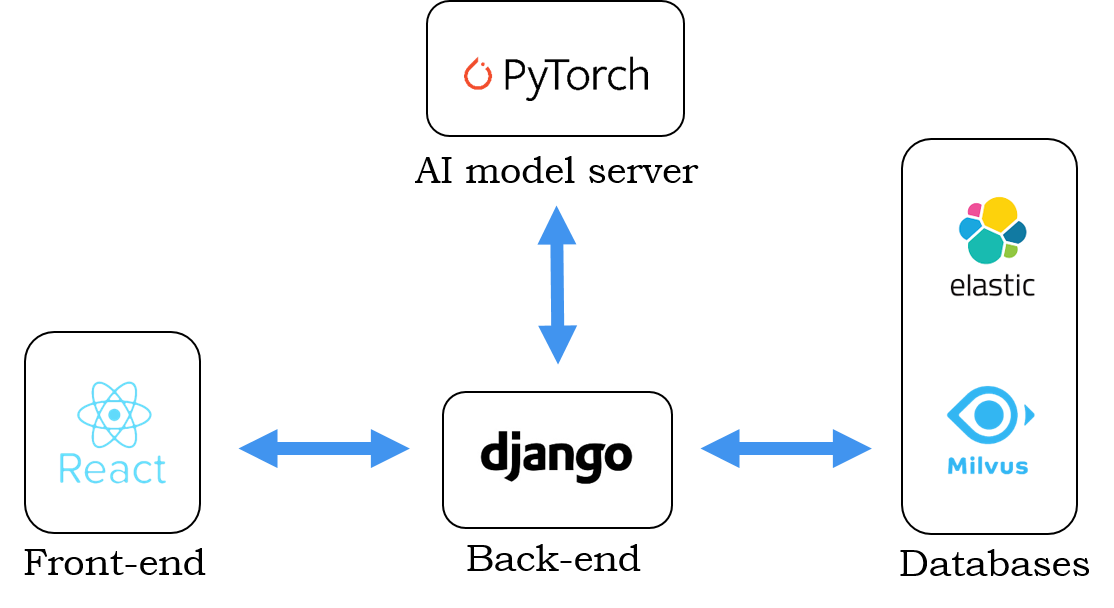
\includegraphics[width=\textwidth]{content/resources/images/methods/architecture.png}
    \caption{The architecture of our application.}
    \label{fig:Retrieval_architecture}
\end{figure}

\section{System design}
\label{sec:first_system_design}

\vspace{-2mm}
We discuss our design principles and highlight some design choices that best express said principles. These principles arise from the motivations discussed earlier in Section \ref{sec:motivation}.

\begin{itemize}
\vspace{-2mm}
    \item \textbf{Flexiblity} \quad As it is present in our system's name, flexibility is the ability to be easily altered depending on the circumstances. This is important to our objective of being a smart system, as it allows countless use cases with the correct modification. For example, using a domain-specific AI model will enable the application to work on that particular domain. To achieve this principle, we have to be clever in architecting our system such that the components are appropriately \textbf{decoupled} in order to allow modifications in functionalities as in the previous example.
\vspace{-2mm}    
    \item \textbf{Scalability} \quad We wish to work with large quantity of data, therefore scalability is essential. It is even more so because we are creating an application, where user experience can be negatively affected with just a slight increase in processing time. To realize this, we need to look beyond everyday AI model development thoughts and borrow ideas from other disciplines, such as software engineering, where there is substantial experience working with applications for the average user.
\vspace{-2mm}    
    \item \textbf{Openness} \quad Though we want our system to have a wide range of features, it cannot be omnipotent and, therefore, will have some areas that it is lacking. To address this, we propose the idea that our system does not compete with other systems, but coexist with them and acts as a complement to each other. For example, while Google does not act on user data, its cosmic knowledge base can be used to find definitions and examples of rare concepts that, in turn, can be used as the starting point for searching in our system.
\end{itemize}

\vspace{-2mm}
We note that these principles do not work in solitary. In fact, improving one can positively affect another. One notable example is that improving flexibility will lead to increased scalability, because when the system is simplified and aptly modularized, it is also easier to scale those components. We have made some design choices that reflect the principles above:

\begin{itemize}
\vspace{-2mm}
    \item \textbf{Separate visual and textual encoders}: Tackling our retrieval problem requires understanding both visual and linguistic modalities. In recent years, encoder-decoder architecture has become popularized, with Transformers\cite{vaswani_attention_2017} architecture dominating in both components. The Transformer architecture contains the multi-head attention mechanism, allowing the model to attend to different input parts. When working with multiple modalities, different works have different approaches when it comes to designing the attention head. Some approaches propose concatenating the visual and textual features and performing attention as if it were a single sequence. This gives good benchmarks results but carries a hidden computational burden at inference time.
    
\vspace{-2mm}    
    We adopt separate visual and textual encoders, which perform attention on each modality separately. The features are mapped into the same subspace, therefore we can calculate their distance as cosine distance. Computing cosine distance is factorizable, therefore we can compute the features beforehand, store them, and perform rapid computation of distances in real-time using vector databases, detailed in the following design choice. In our opinion, the benefit of significantly improving modularity far outweighs the gain in accuracy in this particular case. Furthermore, the accuracy improvement can be regained by using the simple model as a broad filter and then applying the said architecture to a smaller list of candidates.
    
\vspace{-2mm}    
    \item \textbf{Adoption of vector database}: In order to query data efficiently, a compact representation of the data is usually stored and indexed in lieu of the original data. This is a common practice for text-based data, for which various analyzers and indexes exist. However, visual data is often much larger and much more challenging to infer the semantics due to the large domain gap of the underlying representation. For this purpose, artificial intelligence and computer vision have made substantial efforts to create visual features that are much more compact and usable for searching. Nowadays, deep learning models usually embed the image into a smaller subspace (e.g., $1 * 768$) that satisfies the aforementioned needs. However, as these embeddings do not carry explicit meaning on their own (i.e., they are just a vector of floats), it is improbable to index them in ordinary databases. Therefore, vector databases have been created to enable the storage and fast query of vectors based on cosine distance.
    
\vspace{-2mm}    
    In our system, we use Milvus, a vector database that can query millions of vectors in under 100ms (based on our computational resource). To the best of our knowledge, we are among the first team to adopt this for the challenge. Milvus's performance increase is based on technology such as Facebook's FAISS, CPU-specific instructions, GPU acceleration, and more. They are necessary for good performance, yet tedious to implement from scratch. On a higher level, they also implement algorithms such as k-nearest neighbours and quantization-based inverted indexes, which are more suitable for visual data. By leveraging an existing system, we avoid having to implement these features (as many other teams do) while still using the optimal technology for the problem.
    % \item
\end{itemize}

\section{Front-end design}
\label{sec:first_front_end_design}

\vspace{-2mm}
To summarize, our front-end has the following main features:

\begin{enumerate}
\vspace{-2mm}
    \item \textbf{Web application using React}. With this separation of concern, we avoid the widespread problem of AI applications with poor user interfaces (or none at all). The front-end interacts with the back-end via APIs and the web application can be developed without knowledge of the underlying model.
\vspace{-2mm}    
    \item \textbf{Highly optimized for image viewing}. Since our main interfaces are galleries of potentially up to thousands of images, without proper optimization, it is impossible to render them. Slow rendering will prohibit fast searching, therefore we have to reduce the latency as well. To alleviate this problem, we apply a variety of techniques, including pagination, lazy loading, image compression, loading from local storage, and more.
\vspace{-2mm}    
    \item \textbf{Novel Timeline View feature}. In the previous feature, we addressed the \textit{feasibility} of displaying multiple images. However, we also need to consider its \textit{practicality}, i.e., whether the user can gain information by looking at multiple images in succession. We propose a feature that lets the user view a sequence of images with varying levels of detail based on their need. This feature is discussed in detail in Section \ref{sec:timeline_view}.
\end{enumerate}

\subsection{User interface}

\subsubsection{Main search interface}

Our primary search interface is depicted in Figure \ref{fig:FIRST_mainpage}. It consists of the search bar, which is located at the top, the gallery, which makes up most of the interface, and some other auxiliary elements. The gallery shows search results in decreasing order of relevance, from up to bottom, left to right, with the most relevant item at the top left.

\begin{figure}[h]
    \centering
    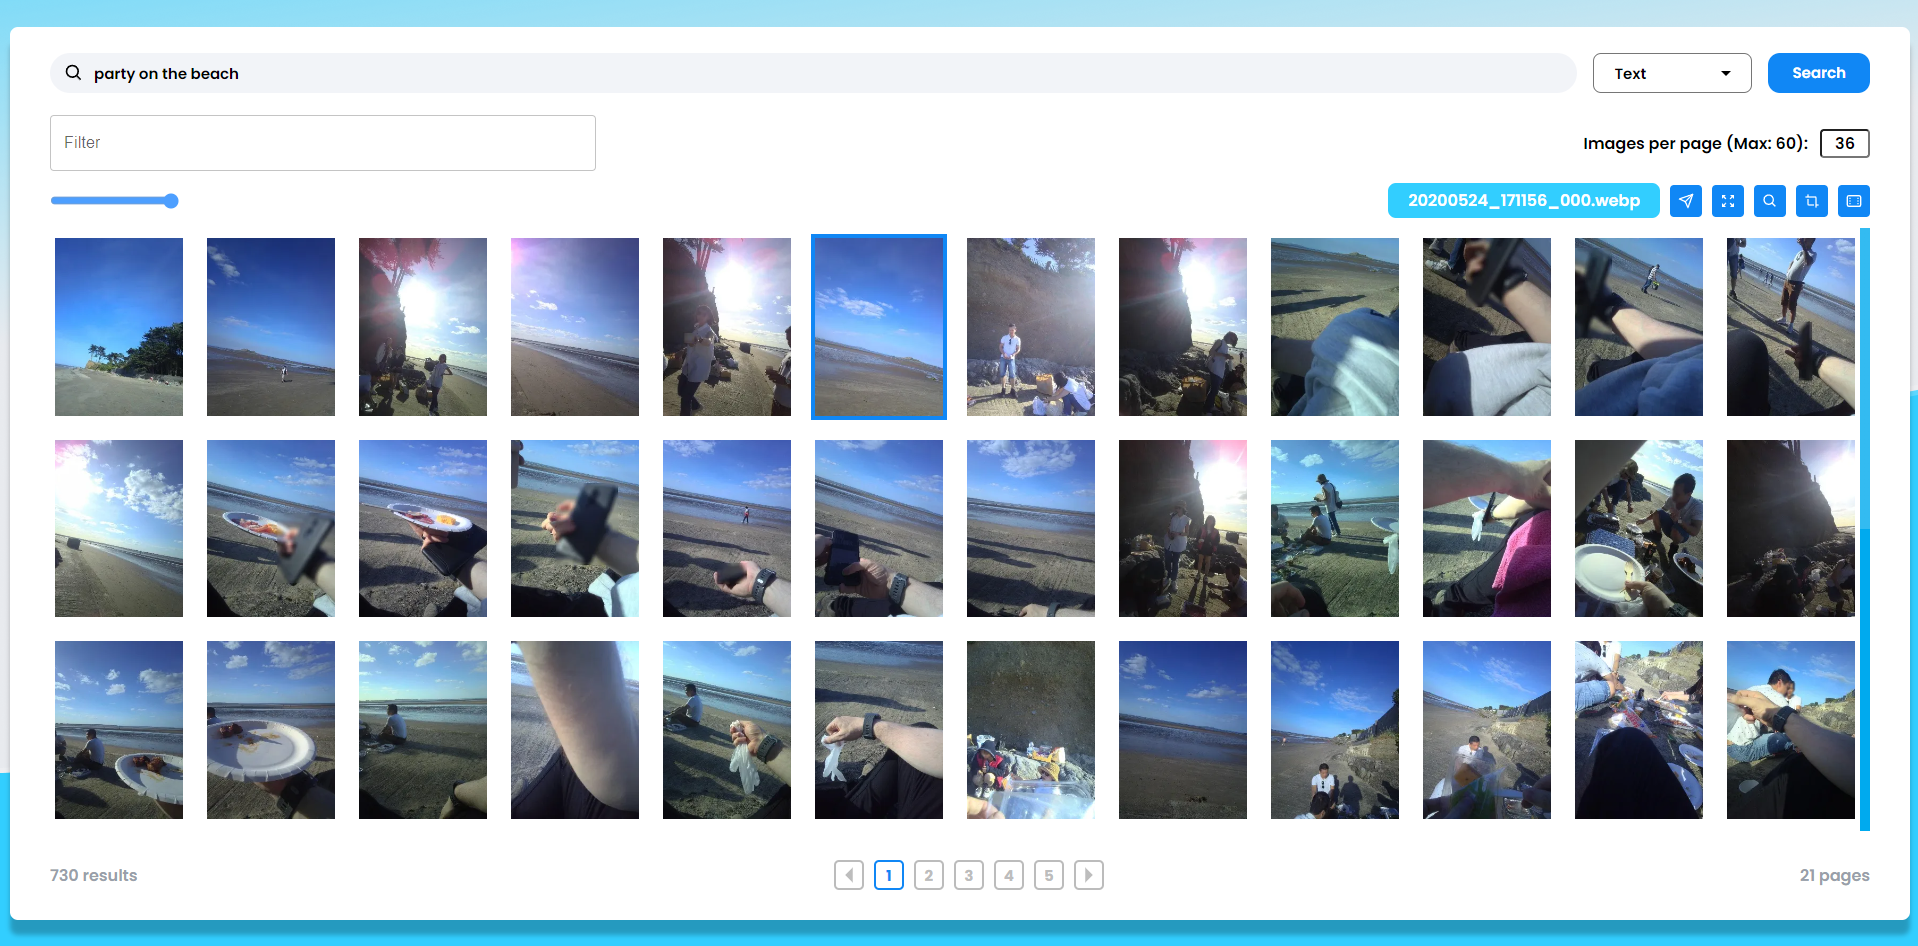
\includegraphics[width=\textwidth]{content/resources/images/methods/FIRST_mainpage.png}
    \caption{The main searching interface of our system.}
    \label{fig:FIRST_mainpage}
\end{figure}

\subsubsection{Timeline View}
\label{sec:timeline_view}

When the user selects an image and chooses the Timeline View function, they will be shown all the images on the same day or in the same video, depending on the use case. The purpose of this function is to allow fast browsing in chronological order to retrieve events that occur before and after a moment. Therefore, when the user switches to Timeline View, which has a gallery view similar to the main interface, there is a button that will quickly scroll to the selected image. If the user wants to look at the image closely, they can switch to Single image mode, which will bring the current image to the middle of the screen and leave only a slider at the bottom. This slider is another way to quickly browse in the time dimension, inspired by the YouTube slider.

Our most notable feature is that we speed up the process of viewing a sequence of images by allowing users to view it with \textbf{varying level of details}. The user can choose to \textit{decrease} the level of detail to quickly find the segment they are looking for, then they can opt to \textit{increase} the level of detail to locate the correct image at \textbf{singe frame precision}. The inner workings of this feature are disclosed in Section \ref{sec:temporal_navigation}.

\begin{figure}[H]
    \centering
    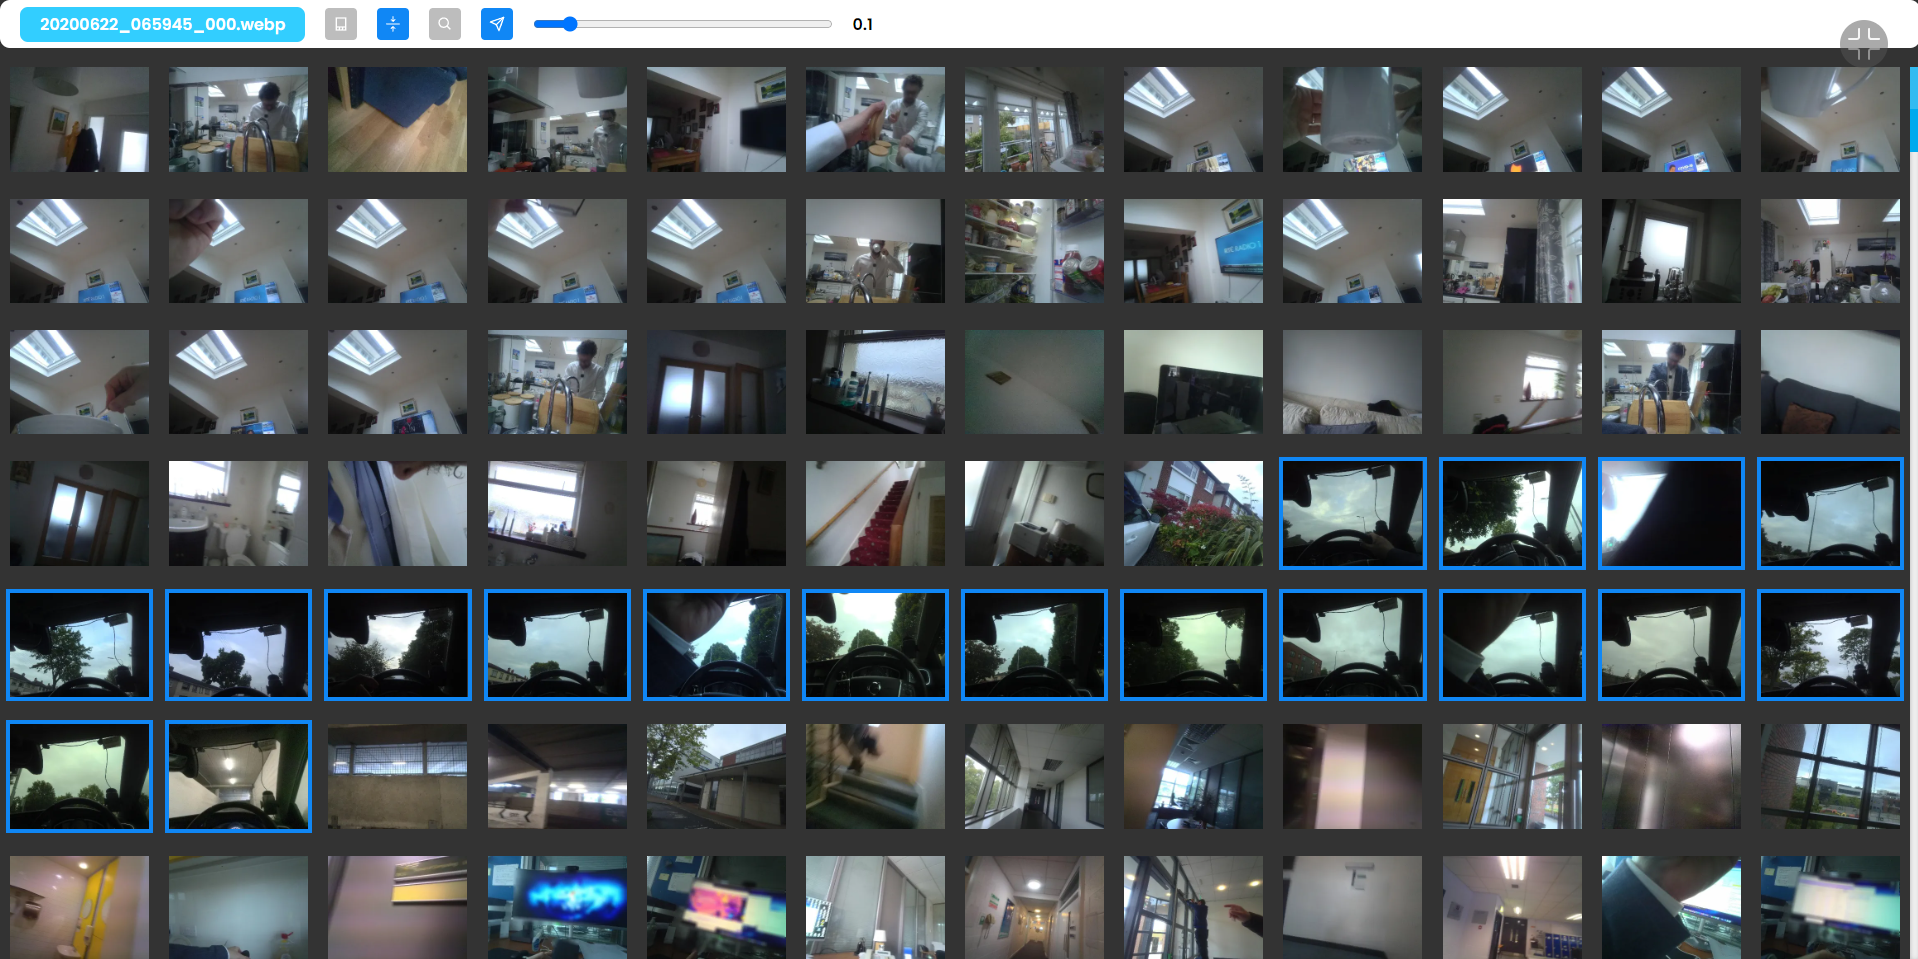
\includegraphics[width=0.9\textwidth]{content/resources/images/methods/FIRST_timeline_before.png}
    \caption{The interface of our Timeline View, gallery mode. }
    \label{fig:FIRST_timeline_before}
\end{figure}

\begin{figure}[H]
    \centering
    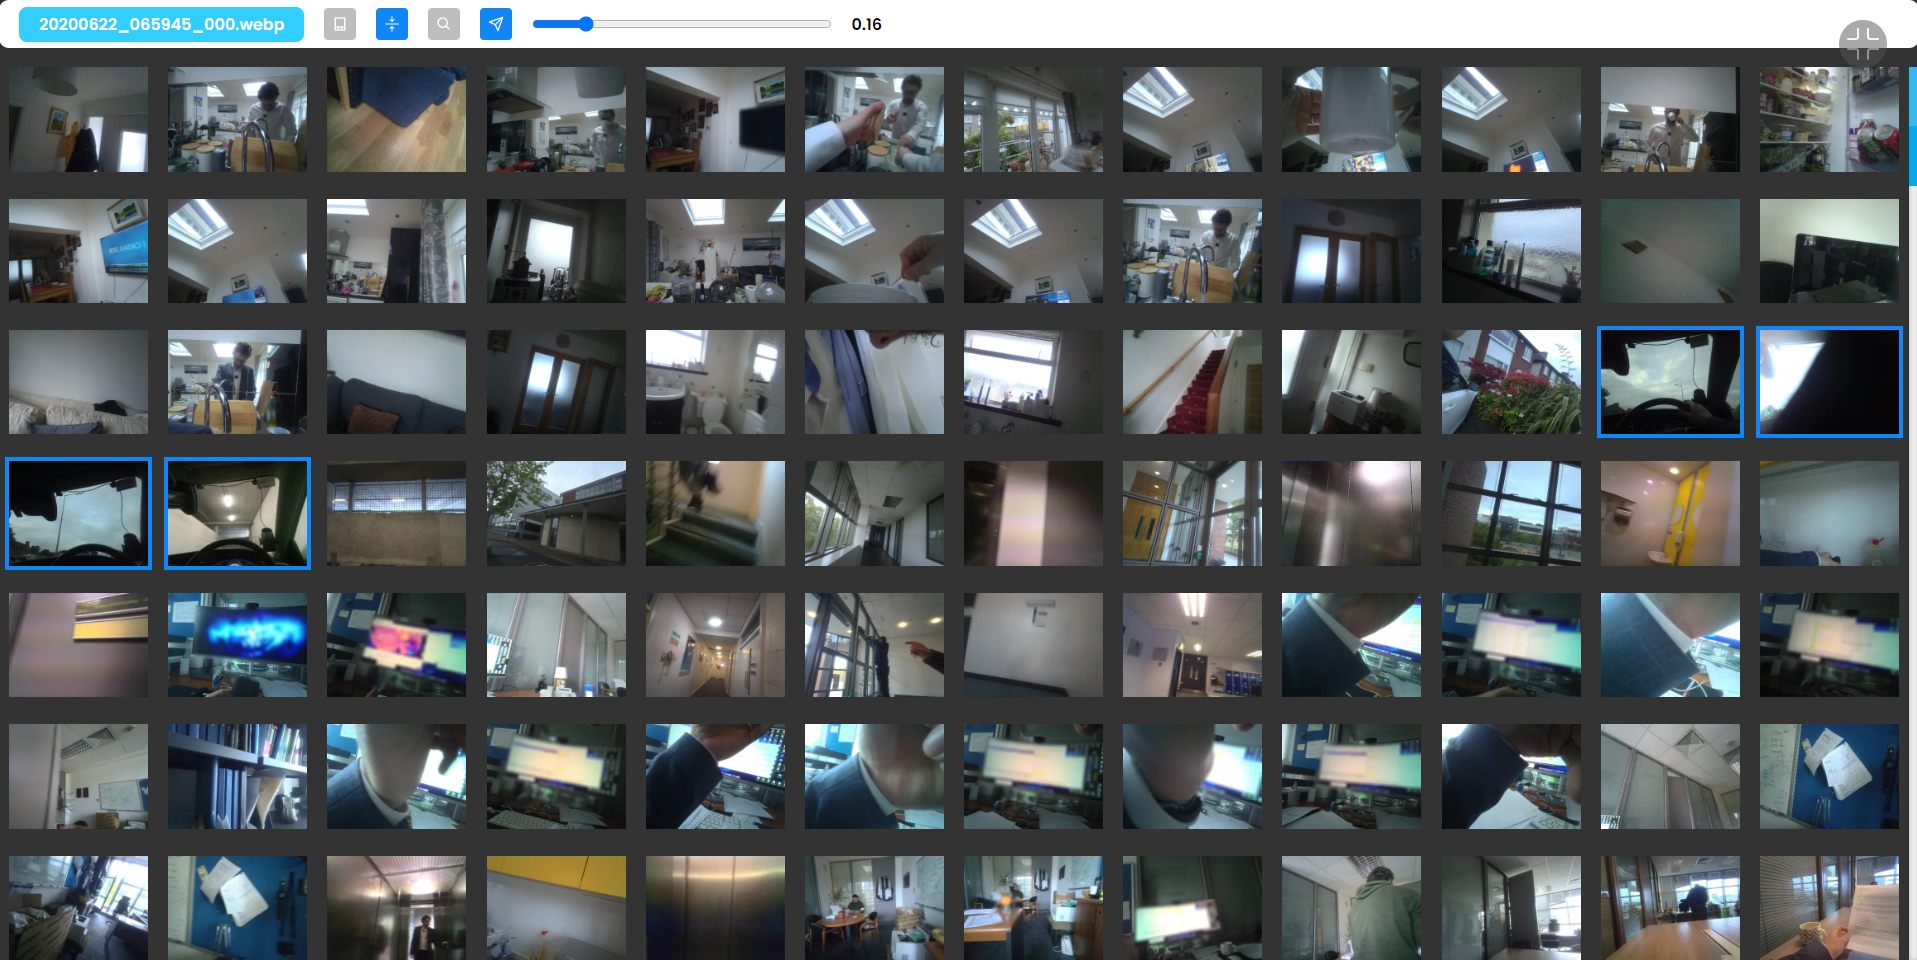
\includegraphics[width=0.9\textwidth]{content/resources/images/methods/FIRST_timeline_after.png}
    \caption{The interface of our Timeline View, gallery mode, with a higher threshold (more concise) than Figure \ref{fig:FIRST_timeline_before}.}
    \label{fig:FIRST_timeline_after}
\end{figure}

\section{Back-end design}
\label{sec:first_back_end_design}

\begin{figure}[h]
    \centering
    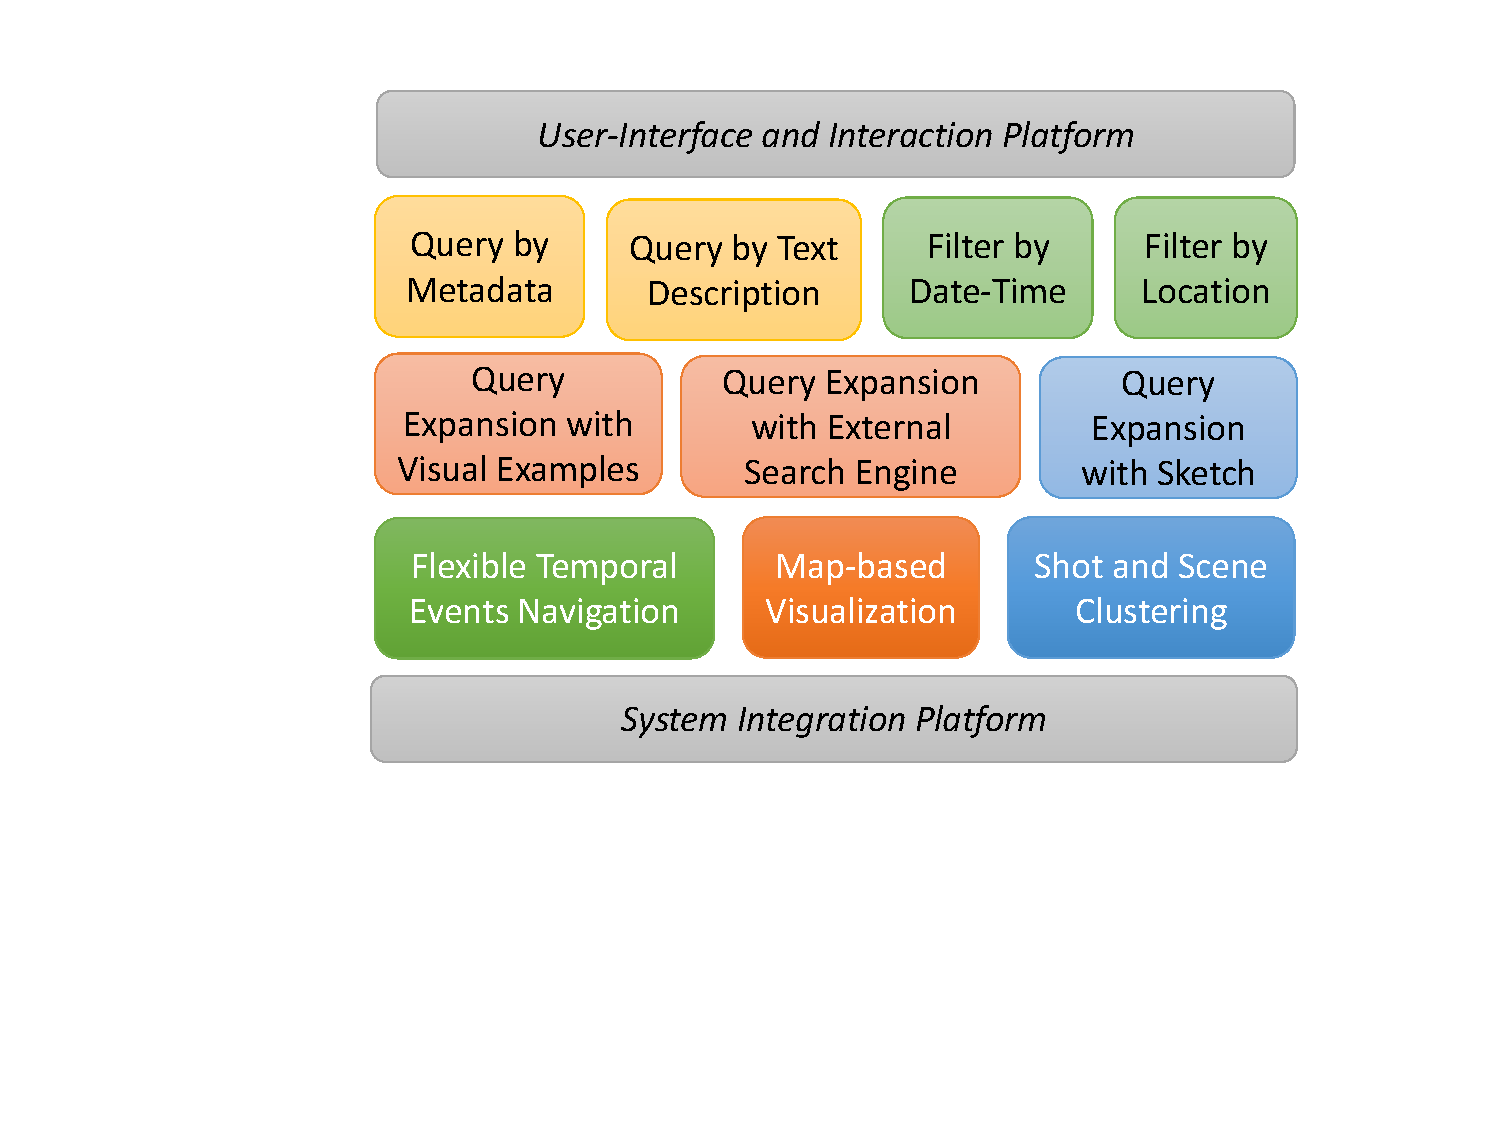
\includegraphics[width=0.8\textwidth]{content/resources/images/methods/FIRST3Components.pdf}
    \caption{Overview of the components of our system.}
    \label{fig:retrieval_components}
\end{figure}

Figure \ref{fig:retrieval_components} shows the overview of the various components in our system, which is developed from FIRST 2.0 \cite{trang-trung_flexible_2021}. The top and bottom layers are platforms on which we can integrate our modules for operational and visualization purposes.

\vspace{-2mm}
\subsection{Efficient clustering of data}
\label{sec:clustering_data}

\vspace{-2mm}
As lifelogging data is periodically taken from the wearable camera every few seconds, they are equivalent to uniform sampling from a video. When dealing with sampled images of this kind, there are a lot of similar-looking images, as the lifelogger cannot always be moving. This phenomenon can be confirmed by looking at Figure \ref{fig:FIRST_timeline_before}, where it can be observed that in a single day, there are lots of consecutive images that are relatively indistinguishable. This is the same situation with videos, as they cannot rapidly introduce new content. Processing the data as-it will result in enormous work with little helpful outcome. For videos, this problem is called the keyframe detection problem, which is challenging on its own. As lifelogging data is not dense enough compared to regular videos (1-2 FPS vs 30 FPS) and spans a much longer time (1 day vs a few minutes), directly applying key frame detection to lifelogging data will be difficult. While coarser sampling can be a quick fix, it can significantly hurt recall, for additional sampling will result in information loss when the sampling is already scarce. 

Besides storage issues, having similar images with no additional information will cause great trouble during retrieval. When an image is deemed relevant, obviously similar images will also be considered such; however since we only return the \textit{top-k} retrieval results, the result will contain many clusters of similar images, which would significantly reduce the variety of the returned results, hindering searching.

We propose a simple grouping strategy to deal with similar images by leveraging the strong expression capability of the visual embedding model used \cite{radford_learning_2021}. We consider images in chronological order and group two consecutive images if their distance in the embedding space is less than a pre-defined threshold. Chains of consecutive grouped images will form \textit{shots}, which we represent with only one image (e.g., the first one) of the shot and discard the rest. This strategy is relatively \textit{safe}, as it only removes very similar-looking images while still preserving slight changes in a small region (e.g., the lifelogger is watching TV), therefore we can be assured that it results in almost no information loss. Though it does not entirely solve the problem, the information density has already increased exceptionally, as we could exclude nearly $30\%$ of the images in the LSC'22 dataset from the vector database using this method with a conservative threshold. 

\vspace{-2mm}
\subsection{Temporal navigation with varying level of details}
\label{sec:temporal_navigation}

\vspace{-2mm}
When we find a relevant image, there is a realistic need to check the preceding/succeeding images to see if the content of the segment agrees with the single image. Some teams seek to implement a feature that allows \textit{playing} the video that contains said image. However, we note that this feature puts a heavy burden on the network and is also not fast enough (the user has to wait for the video to play). Instead, we propose to keep the gallery view and augment it by developing the idea proposed in Section \ref{sec:clustering_data}. While in Section \ref{sec:clustering_data} we cluster the data as a pre-processing step to reduce the amount of data in the vector database, we can simultaneously apply it to shrink the gallery of each day, allowing fast browsing through it and effective usage of screen space compared to the video playing approach. To completely negate the need to view the original data, we need to have varying levels of details, on one side, the user can summarize the sequence to as few as a dozen images, while on the other end of the spectrum, the user can choose to view the original data as-is. Note that even in the latter case, the system only needs to handle all the images in a single day, therefore it still allows for better organization and optimization of data storage. The interface of this feature is depicted in Section \ref{sec:timeline_view}.

\subsection{Attention-based embedding enrichment}
\label{sec:attention_based_embedding_enrichment}

A traditional approach for lifelog retrieval is to extract concepts from an image so that it can be indexed. The extracted concepts can be entities appearing in the image, type of place, type of action, etc. However, this approach depends on the concept detectors for known concepts in a pre-defined dictionary. Therefore, this method is inappropriate for searching for new concepts unavailable in that dictionary.


Keeping in mind the openness of our retrieval system, we aim to represent an image with feature vectors that can be used to match with new concepts. 
For each image in the dataset, we extract a high-dimensional representation using CLIP \cite{radford_learning_2021}. This embedding is a good general descriptor of the image and is close to its main features (concepts). In this way, our system can support users search for simple concepts related to entities in an image (such as \textit{chair}, \textit{TV}, \textit{sandwich}, \textit{etc}) as well as more abstraction concepts (such as \textit{a lecture class}, \textit{a wedding ceremony}, \textit{etc}).

However, the lifelogging data contains very similar scenes in which a subtle change in the image's content can differentiate one image from hundreds of similar ones (e.g., the content of the TV at that time). Therefore, apart from the general concepts in the image, we are also interested in more subtle and local features. 

\begin{figure}[t]
    \centering
    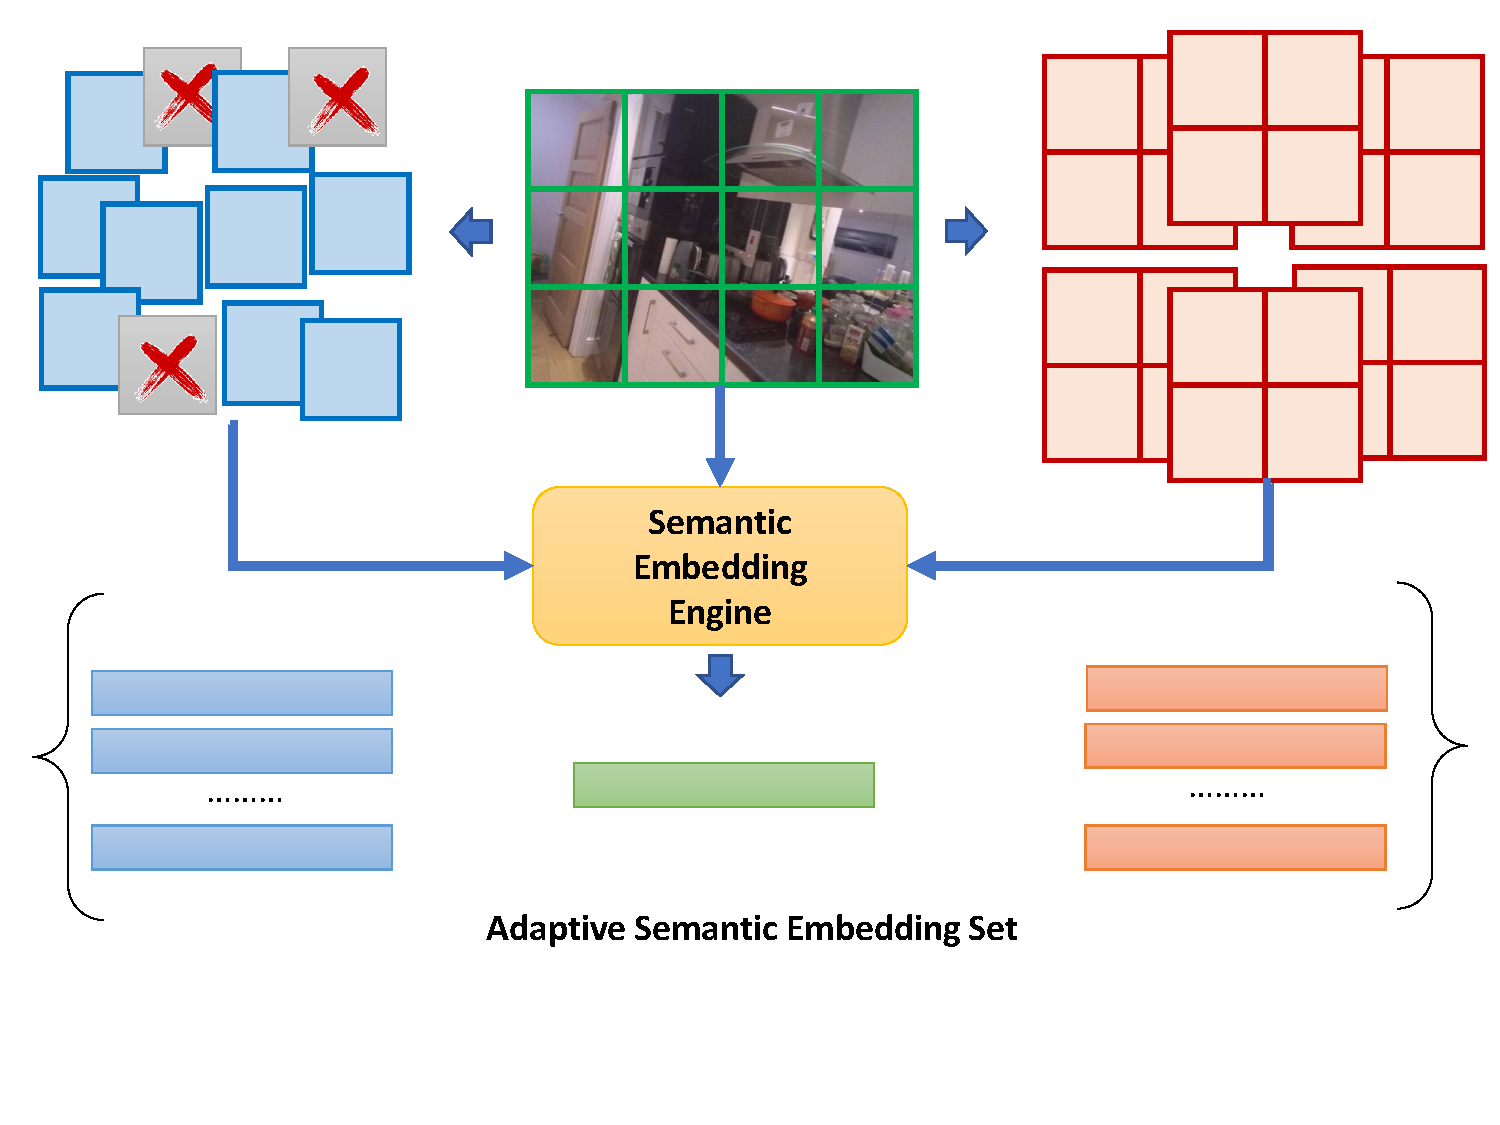
\includegraphics[width=1\columnwidth]{content/resources/images/methods/AdaptiveSemanticEmbeddingSet.pdf}
    \caption{Image decomposition and Adaptive semantic embedding set.}
    \label{fig:AdaptiveSemanticEmbeddingSet}
\end{figure}


Furthermore, since the original size of the images is $1024 \times 768$ and the CLIP model encodes images of size $224 \times 224$ or $336 \times 336$ depending on the model used, they have to be down-sampled in order to be encoded by CLIP, which can cause loss of information. Furthermore, it would not be sufficient to query, \textit{i.e.} to match, an object or concept appearing in a small portion of an image from the global embedding vector of that image. Hence, it should be necessary to encode various important regions of an image at different levels of detail to assist in retrieving different concepts at various levels of granularity in an image.

Due to the above reasons, we seek to add additional information besides the overall image embedding. To achieve this, we select smaller crops of the image and encode them along with the original image. This is similar to the attention mechanic in that we focus on "interesting" regions in the image. The regions to be selected are usually the ones that contain salient objects that can define the scene. This way, we can represent an image with an adaptive semantic embedding set.

Figure \ref{fig:AdaptiveSemanticEmbeddingSet} demonstrates our idea to decompose an image into multiple patches corresponding to different levels of detail and generate an adaptive semantic embedding set corresponding to that image. In our implementation for FIRST 3.0 \citeown{hoang-xuan_flexible_2022}, for simplicity, we represent an image (with the aspect ratio of 4:3) as a grid with $4 \times 3$ square cells. Then we construct multiple patches with the size of $1 \times 1$ and $2 \times 2$ cells, which can be overlapped. Finally, we remove unimportant patches and encode information-rich patches into semantic embedding vectors. The adaptive semantic embedding set is the collection of semantic embedding vectors of the full-size image and its exciting patches.

\subsection{Visually similar image searching}

As stated in Section \ref{sec:first_system_design} in the principle of \textit{Openness}, we use similarity modelling to extend the capabilities of our system. This is a feature that many other methods also seek due to its usefulness in the retrieval setting \cite{nguyen_lifeseeker_2022} \cite{lokoc_enhanced_2021}. In our system, we leverage the strong representational capability of CLIP \cite{radford_learning_2021}, which is demonstrated to be effective even in the zero-shot setting \cite{portillo-quintero_straightforward_2021}. Because CLIP was trained on image-caption classification task, which is a form of contrastive training, we believe it has learned to differentiate between images based on the concepts existing in the images, and so it can encode the image regardless of the content. More importantly, this allows us to simply define the distance between two images as the cosine distance between their embeddings. With this definition, we can quickly find an image similar to a given image in a database. This gives rise to the ability to search using visual examples.

In multiple cases, there are some concepts that cannot be well described using words, are unknown to the user, or are unavailable in the training corpus for the text encoder. Such instances are present in previous editions of the LSC. While trying to expand the pre-defined dictionary helps in all cases, it requires much effort to identify the needed concepts and also comes with storage and computing costs. We deviate from this paradigm by two means: utilizing \textit{external} systems and modelling \textit{deep} image semantic.


\begin{figure}[]
    \centering
    \vspace{-2mm}
    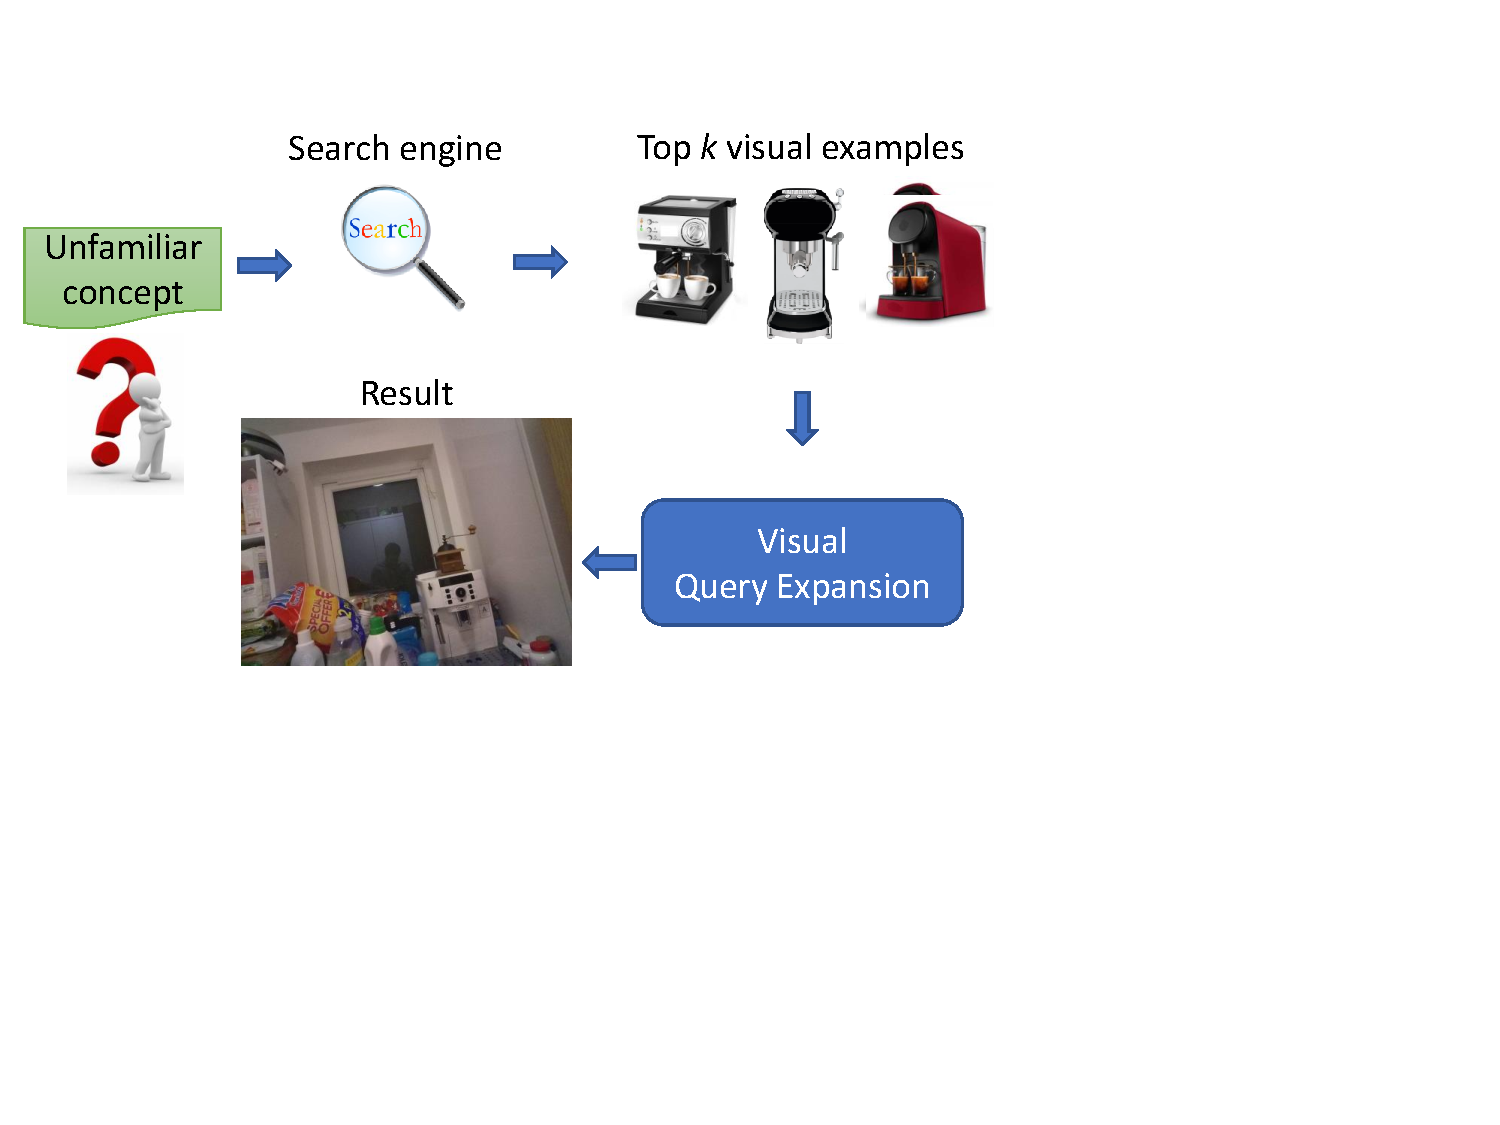
\includegraphics[width=0.9\columnwidth]{content/resources/images/methods/VisualQueryExpansion.pdf}
    \caption{Retrieval of an unfamiliar concept with the assistance of visual search engine.}
    \label{fig:VisualQueryExpansion}
\end{figure}

With the ubiquitous amount of data available on the Internet, we believe that any possible concept, possibly along with an image-text correspondence, exists and can be found with an appropriate tool, such as Google Search. We can query those tools to find an example of such a concept and use it as a starting point for our retrieval process. With our visual comparison capabilities mentioned earlier, we support the use of an external image as a prototype for query, as demonstrated in Figure \ref{fig:VisualQueryExpansion}. We can look for \textit{coffee machine} with visual examples suggested by an external search engine. This approach allows us to broaden the scope of searching beyond our existing concepts and utilize the strengths of other systems while producing a natural and intuitive searching process. This feature works well with our adaptive embedding described in Section  \ref{sec:attention_based_embedding_enrichment}, as the particular unknown/unfamiliar concept usually only occupies a portion, or even a tiny bit of an image, and therefore focusing on it greatly helps with "matching" it to the available prototype.

Many works \cite{tran_e-mysce_2022}, \cite{trang-trung_flexible_2021} enrich images with metadata tags from pre-trained state-of-the-art object detectors. While this is intuitive and effective, and we do this ourselves too, we propose a further advancement by modelling more abstract concepts from the image, such as events. This can be achieved in a number of ways, one of them is breaking down or associating an abstract concept with simple concepts or objects that can be searched for. An example of this is that instead of searching for "teaching", which is difficult to define, we can try to look for whiteboards, people in a room, desks, etc. As another avenue, we note that recent advances in representation learning have made this more possible than ever; we show that since CLIP was trained on image-caption pairs, it has some (limited) ability to understand a scene in the same way a human does. We can directly leverage this to empower our searches. By leveraging general representations instead of task-specific representations, advances to these models also empower our search engine without intervention. We believe this direction may prove useful and make future search engines simpler yet more powerful.

% \subsection{Query expansion via pseudo relevance feedback}

\section{Lifelog Search Challenge 2022}

The Lifelog Search Challenge (LSC) provides an opportunity for developers to qualitatively and quantitatively benchmark their system, both through expert and novice users, on a common dataset in a common setting. It has been organized every year since 2018 as an offline workshop, with the exception of 2020 and 2021 due to the COVID-19 pandemic. By gathering all systems and evaluating on the same dataset and queries, it is possible to benchmark the performance of different systems fairly. Furthermore, the assembly also facilitates the exchange of ideas and discussion of problems and potential solutions, gradually improving the quality of participating systems and the challenge as a whole.

In its 5th iteration, the LSC'22 was held in a hybrid format in Newark, New Jersey, as part of the ACM International Conference on Multimedia Retrieval (ACM ICMR'22). Our participation was online due to difficulties in applying for a U.S. visa.

\subsection{Dataset}

The LSC'22 dataset is recorded by a lifelogger using a wearable camera 24/7. The dataset consists of approximately 750000 images, spanning a time period of 18 months, and taking up storage of 44 GB. The dataset is fully anonymized and redacted before publication: faces and sensitive texts were identified and blurred, while sensitive scenes were filtered and deleted. 

\subsection{Query format}

The search topics are divided into 3 categories for LSC'22:

% And finally, since everyone has taken part in a testing session, we all know the query types, but just to remind everyone:
% - KIS Topics - Find one relevant item from the collection to match the temporally increasing query. Total time is 5 minutes. Standard VBS / LSC KIS scoring is used here which penalises incorrect submissions. These are automatically judged against a pre-calculated list of correct items. If there is a dispute over a topic, we can evaluate a disputed item after the topic (in the competition).
% - Ad-Hoc Topics - Find as many relevant items as possible with a 3 minute time period. Each of these have to be judged in real-time, so these will take time if a lot of submissions are made.  For VBS participants, this is similar to the textual AVS task.
% - Q&A Topics - The idea here is to find one correct answer to the topic. You are only allowed to submit one answer, which will be judged correct or incorrect. There is a 3 minute time limit on this type of topic. This is scored as a KIS task, so time to find the item is important.

\begin{itemize}
    \item \textbf{Known item search (KIS)} - This topic requires participants to find the one relevant image from the collection. Participants will be given a textual description of the item, and more clues will be gradually revealed over a period of 5 minutes. The scoring will be based on how soon the team finds it and the number of incorrect submissions. 
    \item \textbf{Ad-hoc topics (AD)} - This topic demands as many relevant items as possible within 3 minutes. Unlike KIS, the topics are usually much broader (e.g., "find all images of toy trains"). Since there can be diverse answers, the submissions are judged manually.
    \item \textbf{Question answering (QA)} - Originating from the need of automatic question answering systems, this topic allows only a single submission to address a particular information need (e.g., "what is my house's number?"). The submitted image should explicitly contain this information, and it will also be manually judged.
\end{itemize}

One of the actual queries for LSC'22 was: \textit{I think it was the second time I visited a stone shed. The shed was under green trees. It takes 2 hours to drive there and 2 hours back. It was in May 2020.} The answer can be found in Figure \ref{fig:LSCsample}. As can be seen, the prompt consists of multiple sentences, each shown gradually one after another, each revealing additional information (\textit{stone shed}, \textit{under green trees}, \textit{driving}, \textit{date}). The participant has to selectively combine all of this information to locate the answer in the shortest time possible.

\begin{figure}[h]
    \centering
    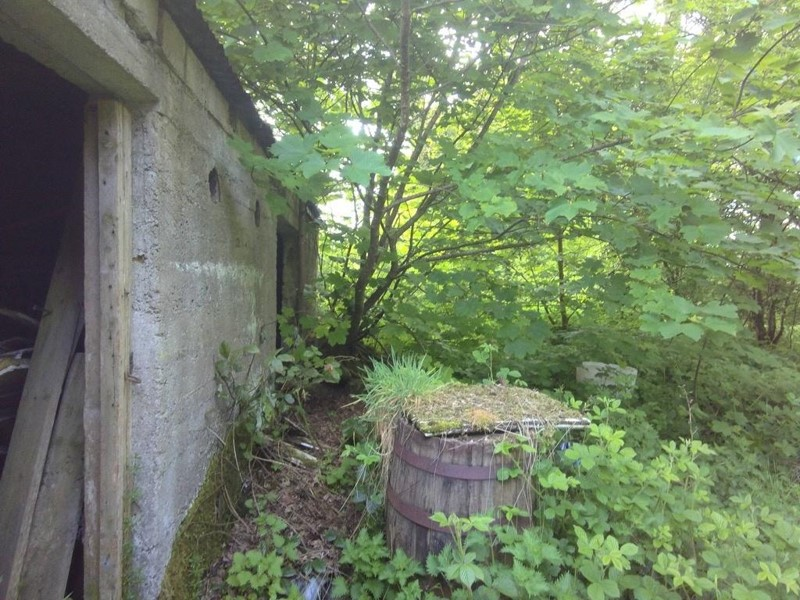
\includegraphics[width=0.6\textwidth]{content/resources/images/evaluation/LSCsample.jpg}
    \caption{Sample answer for an actual query at LSC'22.}
    \label{fig:LSCsample}
\end{figure}

\vspace{-2mm}
\subsection{Evaluation method}

\vspace{-2mm}
For the LSC, one of the judges, who is also the lifelogger that records the dataset, will generate queries based on their memory. Teams will be tested on a (possibly uneven) number of topics of all three categories during the workshop session, in no particular order. 

\vspace{-2mm}
The participants will view the queries and submit their answers via the DRES system. The scores will be separate for each category, with the final score being the sum of each category. Within each category, the scores are normalized such that the top performing team's score is always 100. The particular scoring functions for KIS and ad-hoc topics are different, and QA topics are judged as KIS topics.



\section{Visual Browser Showdown 2022}

The Video Browser Showdown (VBS) is a long-time video search competition with the goal of developing fast and effective video search systems. It has a very similar format to the LSC; in fact, it is the LSC that is based on the VBS competition as it has been around since 2012 as part of the International Conference in Multimedia Modeling (MMM). The VBS works with general video data, unlike the LSC, which is focused on lifelogging. Many teams participate in both VBS and LSC because they are similar in format, and at the same time, each competition presents a different challenge that they can evaluate their system on.

For the 2022 edition, the Visual Browser Showdown 2022 (VBS 2022) challenge was held in Phu Quoc, Vietnam, in conjunction with MMM 2022. While the conference was held in a hybrid format, we took the chance to participate on-site.

\subsection{Dataset}

The VBS competition shares the same dataset with TRECVID (\textbf{T}ext \textbf{RE}trieval \textbf{C}onference \textbf{VID}eo Retrieval Evaluation), a workshop sponsored by the National Institute of Standards and Technology (NIST) also working information retrieval research. The dataset used for VBS 2022 is V3C1 and V3C2 combined, which amounts to 17235 videos, totalling approximately 2300 hours and 3 TB of storage. The dataset is based on Vimeo, an online video-sharing platform similar to YouTube.

\subsection{Query format}

VBS 2022 features very similar search topics to LSC'22, with minor differences. Note that VBS works with video data, therefore the search target for KIS tasks is a short segment (usually under a minute) of a video that contains the event(s) described by the prompt.

\begin{itemize}
    \item \textbf{Known item search - Text (KIS-T)} - This topic is the same as LSC known item search. However, since the VBS data is not lifelogging data, the description is focused on the people, objects, and scenes present in the video, without information such as time.
    \item \textbf{Known item search - Video (KIS-V)} - For this topic, a short segment of a video is given, and participants are asked to locate it (i.e., find the video id and its timestamp). Everything else is the same as KIS-T tasks. 
    \item \textbf{Ad-hoc topics (AVS)} - This topic demands as many relevant items as possible within the time limit. Note that in this topic (and all other topics), image submissions are expected.
\end{itemize}

\subsection{Evaluation method}

The queries are generated by the judges prior to the competition, as with LSC. Scores are separately normalized for each category, and the overall result is the sum of each category.

\section{Interactive Retrieval Results}

We report the benchmarks of our system from LSC and VBS competition, in addition to detailed analysis of overall performance and case study. From experience we gained during the development and actual usage of the system, we sum up some best practices for novice and intermediate users to make the most of our system.

\subsection{LSC'22}
\label{sec:LSC22}

\begin{figure}[h]
    \centering
    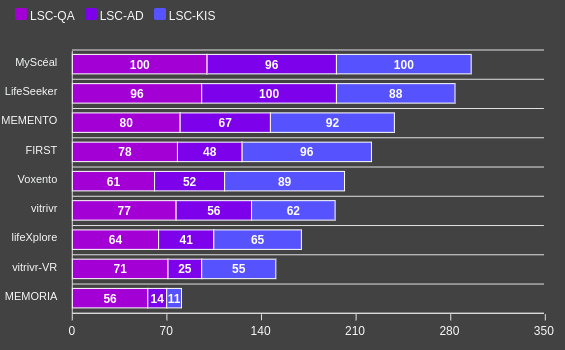
\includegraphics[width=\textwidth]{content/resources/images/evaluation/LSC2022_results.png}
    \caption{Result of all teams at LSC'22. Our team's name is FIRST.}
    \label{fig:LSC2022_results}
\end{figure}

At LSC'22, we placed 4/9, winning Best KIS (after overall winner MyScéal). The breakdown of all categories for all teams can be found in Fig \ref{fig:LSC2022_results}.

As our system is designed with KIS in mind, overall, our system performs best within that category. QA is a new category that requires ancillary tools (e.g., a map), while AD tasks require detailed processing of the original videos.

\subsection{VBS 2022}
\label{sec:VBS2022}

\begin{figure}[h]
    \centering
    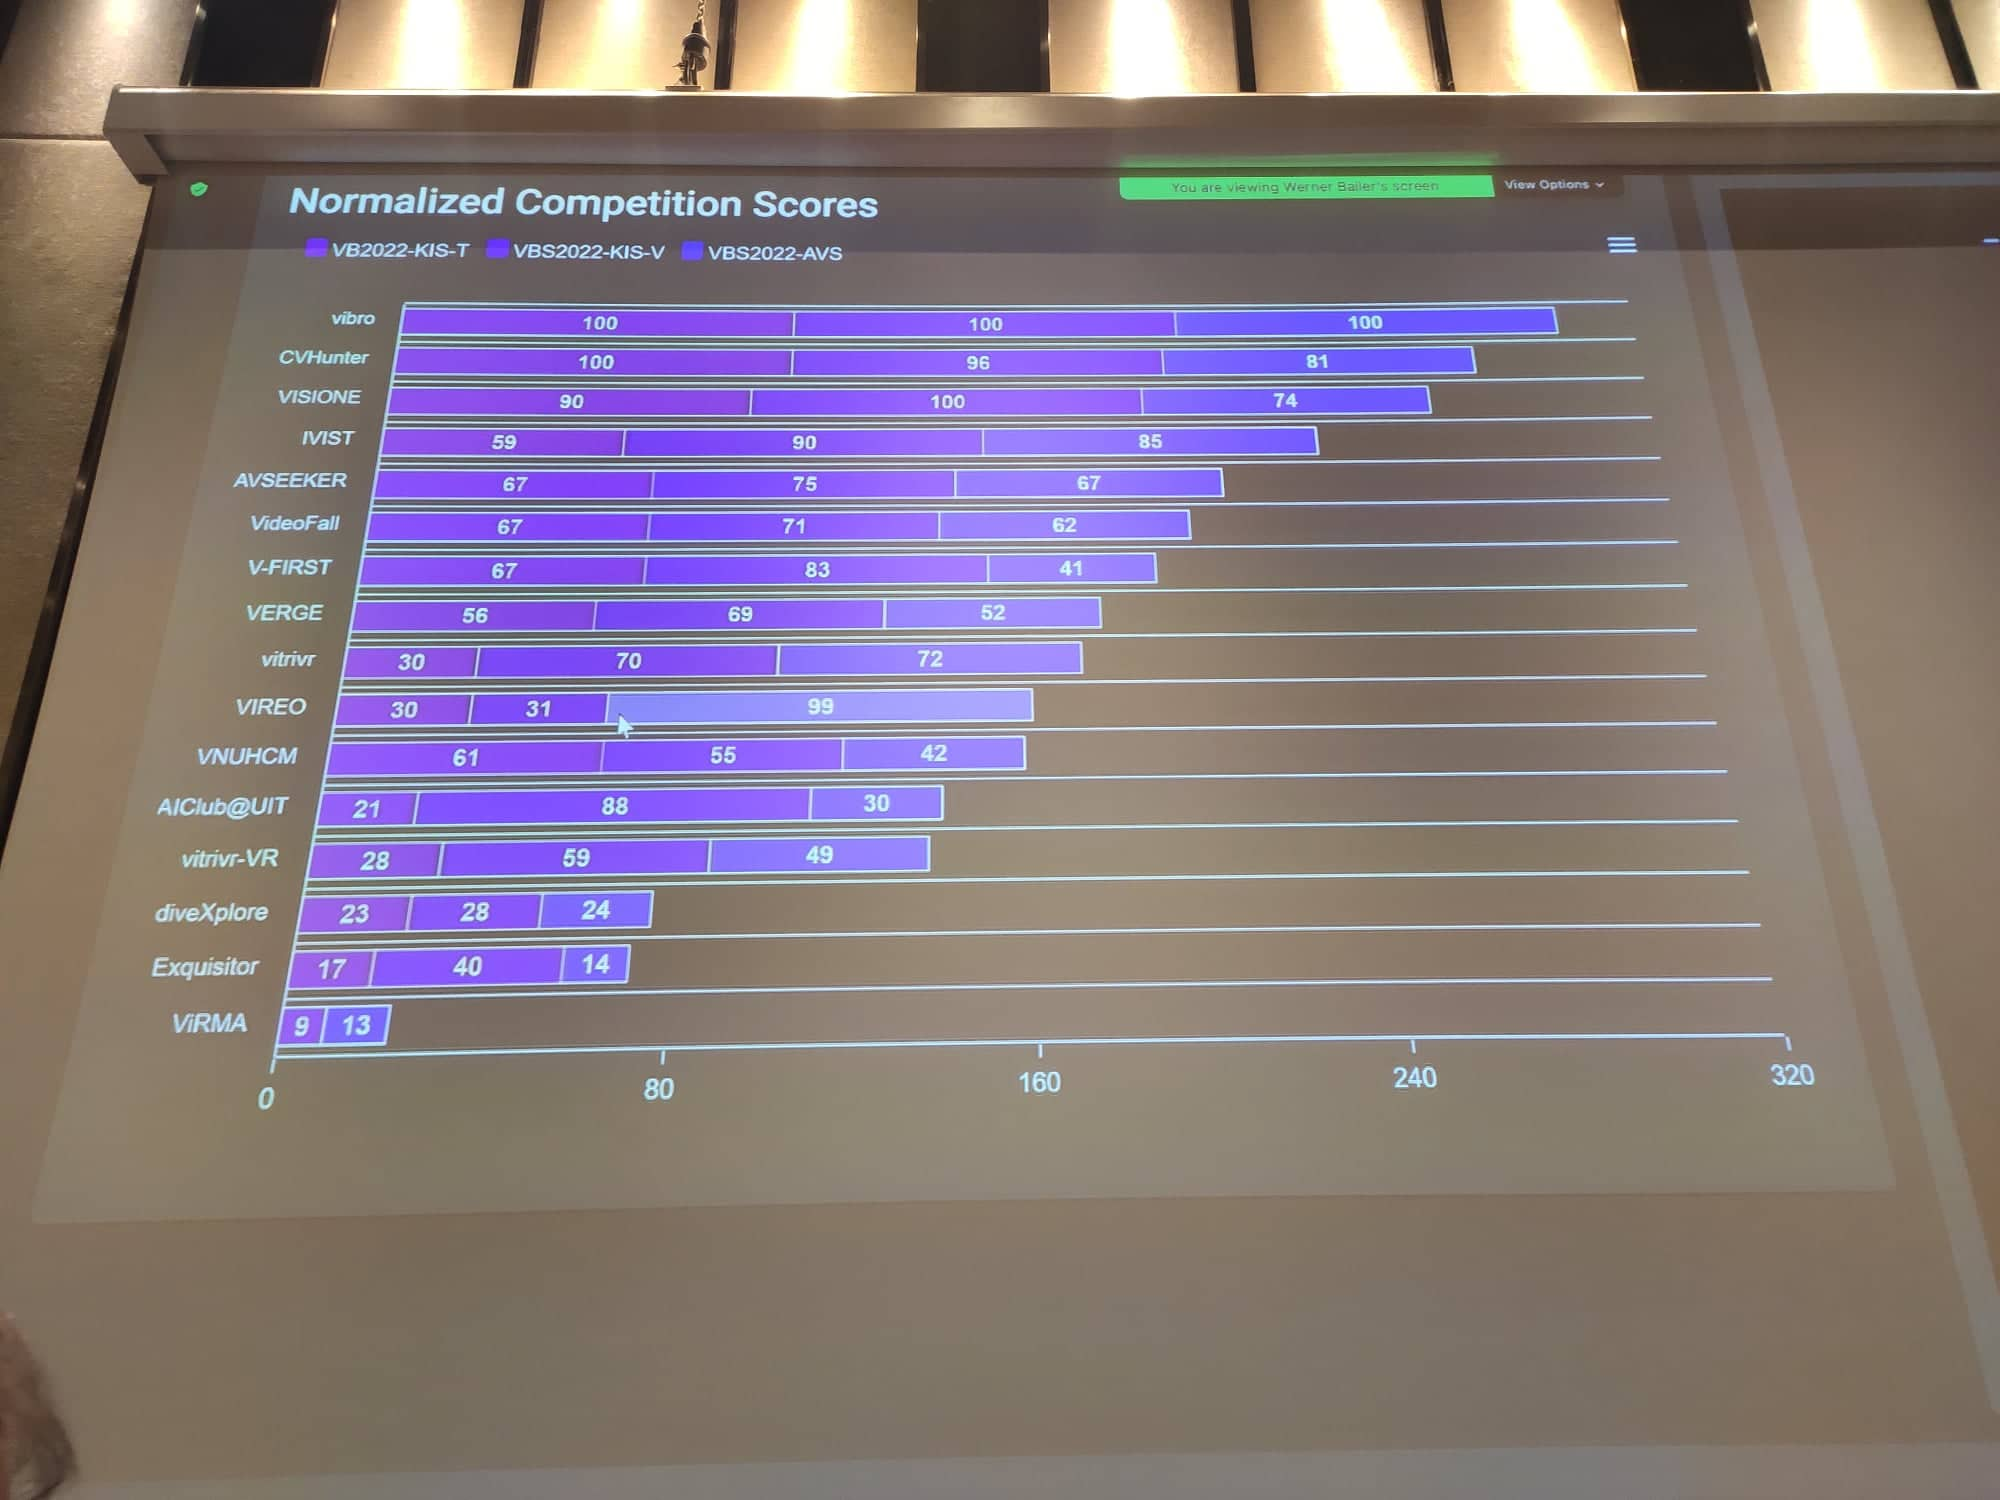
\includegraphics[width=\textwidth]{content/resources/images/evaluation/VBS2022_results.jpg}
    \caption{Result of all teams at VBS2022. Our team's name is V-FIRST.}
    \label{fig:VBS2022_results}
\end{figure}

At VBS 2022 \citeown{tran_v-first_2022}, we placed 7/16, just a bit behind Best Newcomer VideoFall. We scored 67 on KIS-T, 83 on KIS-V, and 41 on AVS. The detailed results can be seen in Fig \ref{fig:VBS2022_results}.

\subsection{Case study}
\label{sec:CaseStudy}

% 1: removal of repetitive scenes allow for varied results: lighting fixture 
% 2: focus on local content: TV content
% 3: image searching: pendant lamp


% example: 20190101_140454_000

\vspace{2mm}

In this section, we describe some specific usage scenario to demonstrate how to best use our system, as well as its strengths.



\textbf{Scenario 1:} \textit{I was looking at a lead soldier in a mall, next to some clothes.}

We think of two strategies to approach this query, either directly searching for "\textit{lead soldier}", or imagining a typical lead soldier and trying to describe it. For the second strategy, we might attempt to look for a standing man, wearing a red shirt and a top hat. 



\begin{figure}[h]
    \centering
    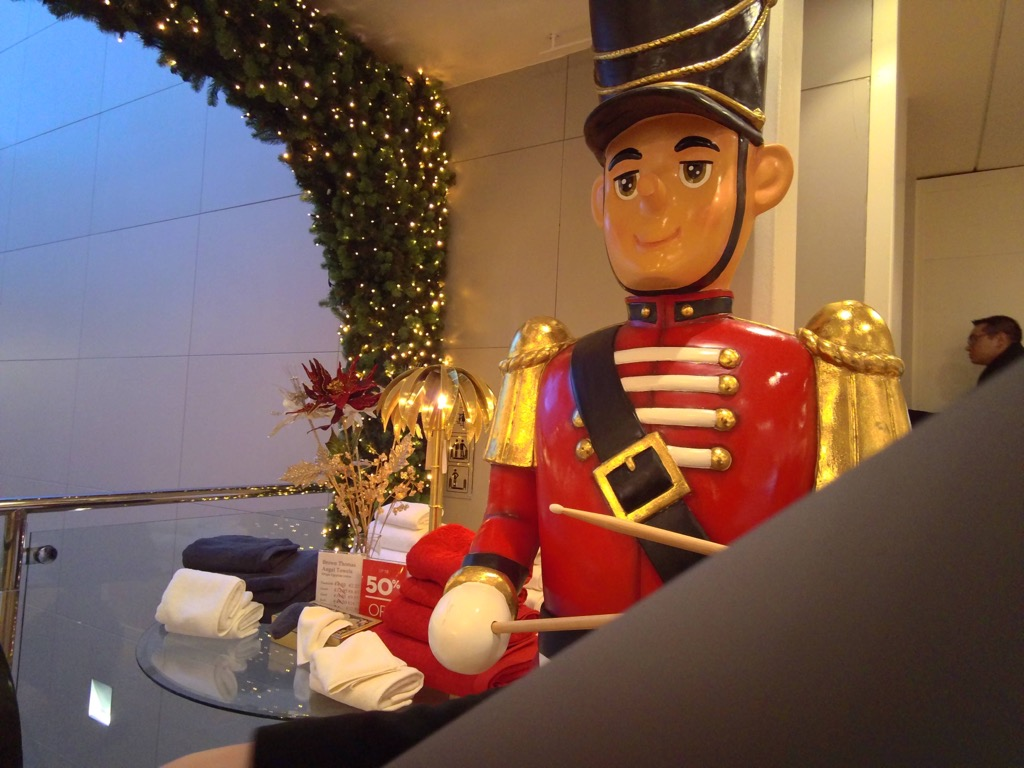
\includegraphics[width=0.7\columnwidth]{content/resources/images/methods/CaseStudy1Target.jpg}
    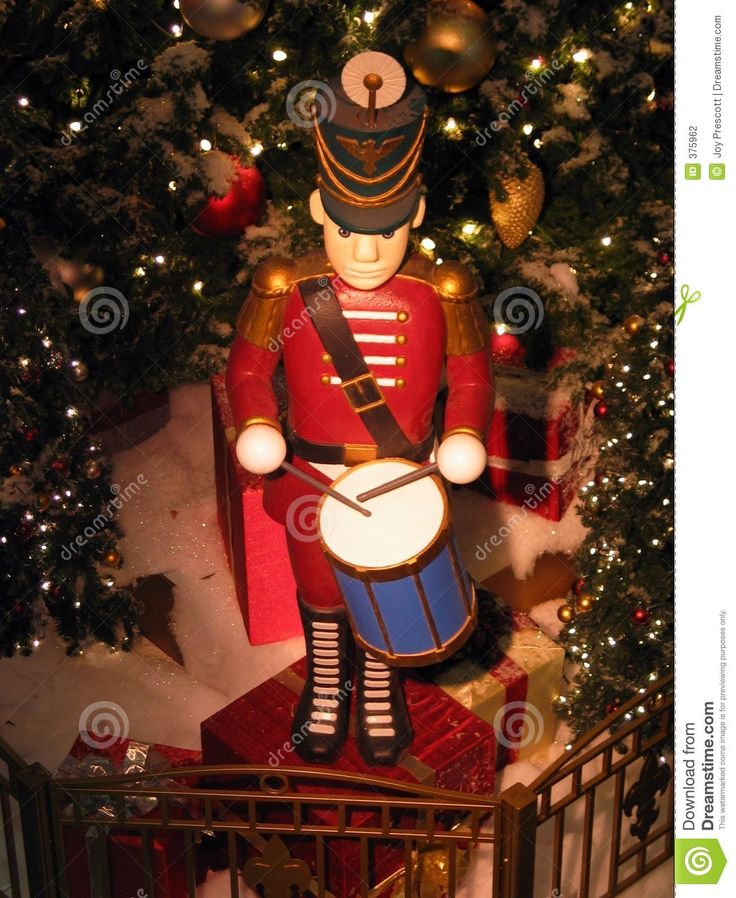
\includegraphics[width=0.25\columnwidth]{content/resources/images/methods/CaseStudy1Prototype.jpg}
    \caption{The first scenario. The target image is on the left, while the image on the right is the prototype we took from Pinterest.}
    \label{fig:CaseStudy1}
\end{figure}

The results of both approaches are shown below.
\begin{itemize}
  \item[] a lead soldier standing \xmark
  \item[] a lead soldier wearing red shirt \xmark
  \item[] a lead soldier wearing red suit \cmark
  \item[] a man wearing red suit \xmark
\end{itemize}



We observe that searching for "man" or "red suit" yields too many results and not the one we are looking for, and even in the query that successfully found the target image, the results are inconsistent. Instead, we can search for a concrete example on the Internet and use it directly for our search, as shown in Figure \ref{fig:CaseStudy1}. This gives the target image as the top-2, and at the same time, yields two other images with a lead soldier in it in the top-15, which none of the shown queries was able to. As mentioned above, we only need the URL of the image, so the process is fairly quick and much faster than the try-and-error approach of query engineering.




\textbf{Scenario 2:} \textit{I was taking a photo of a man sitting at a table. I took a flight to this city 3 days ago. I was in Greece then.}

\vspace{-2mm}
In this example, we would like to illustrate our system's capability to retrieve a moment with the activity or story in an image, instead of looking for only entities/objects appearing in it. With the first sentence in the query description, rather than looking for the moment when we can see a smartphone or camera in a photo, we can simply search with the text description "\textit{I was taking a photo of a man sitting at a table}". 

\vspace{-2mm}
If there are multiple moments, we can verify the event of interest using the second sentence in the query. Three days can be a long duration and it would be inconvenient and inefficient for a user to navigate through a long sequence of images just to verify the previous event of taking flight and arriving at a new city. Our system assists users with a flexible navigation mechanism and grouping similar images into shots, thus the system helps users quickly confirm the moment happening 3 days ago. 

\begin{figure}[t]
    \centering
    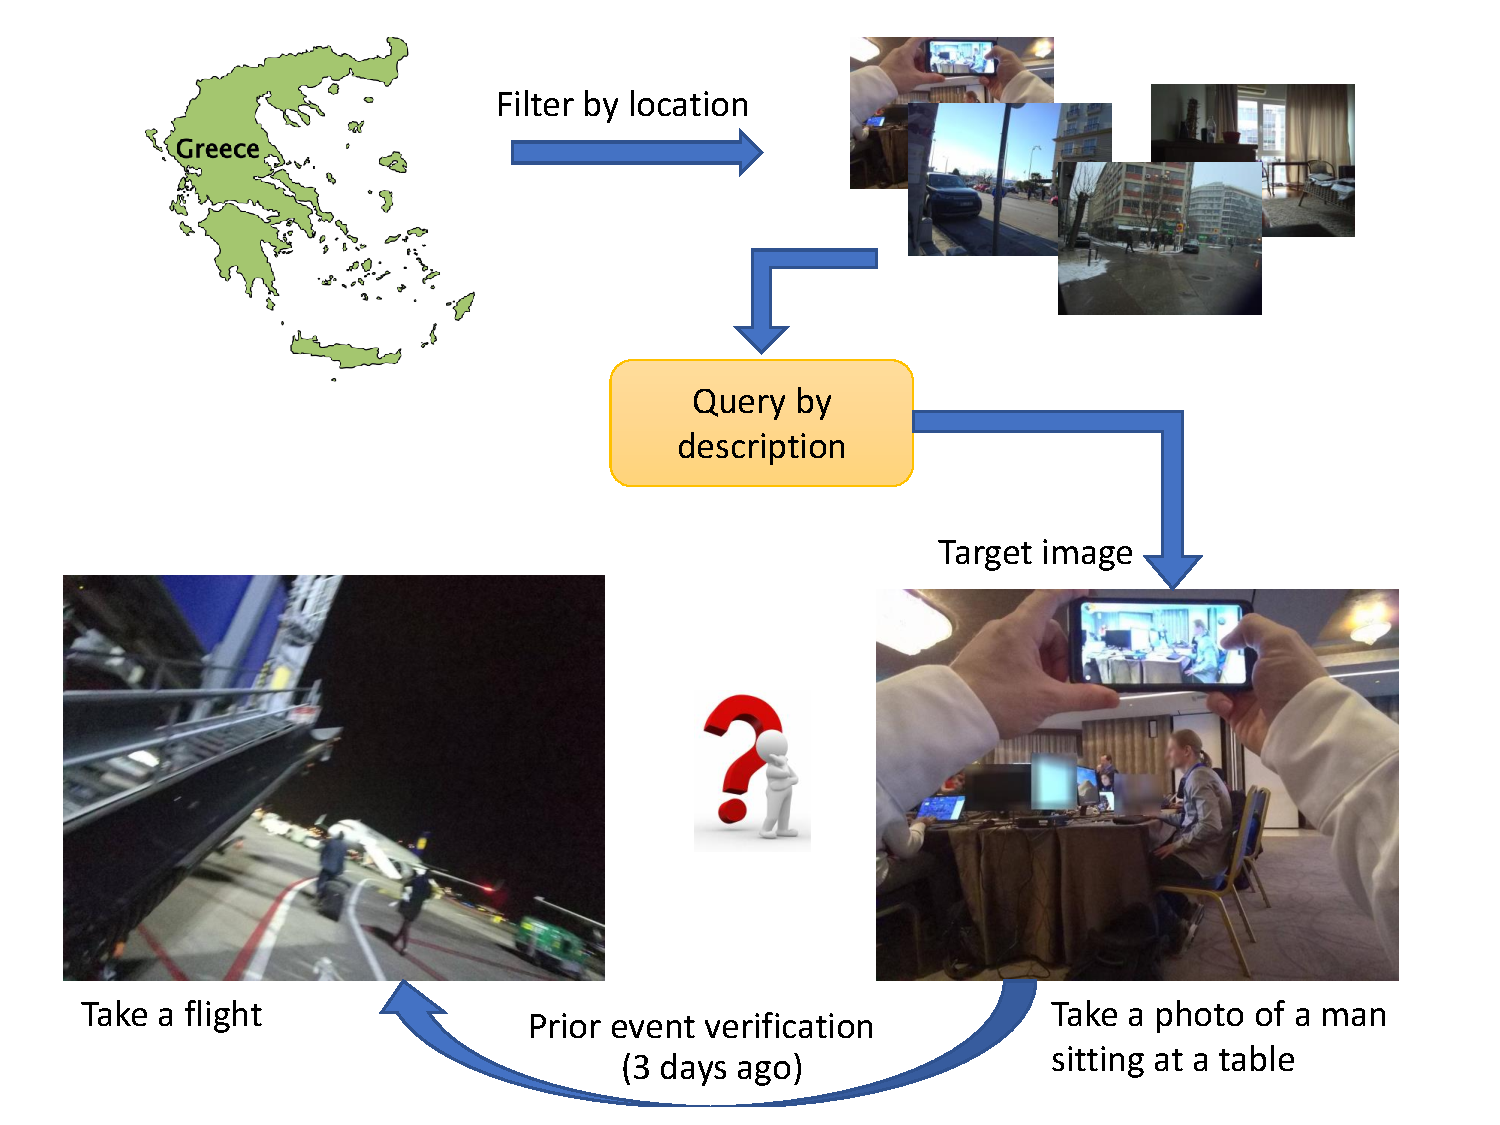
\includegraphics[width=1\columnwidth]{content/resources/images/methods/CaseStudy2Overview.pdf}
    \caption{The second scenario. The target image can be identified from description, location filtering, and prior event verification.}
    \label{fig:CaseStudy2}
\end{figure}

\vspace{-2mm} 
Finally, if we wait until the last minute to exploit the last sentence in the query description, we can narrow down the moments occurring in Greece. We can simply set the filter on the location ("\textit{in Greece}") and query with the description from the first sentence, and we can successfully identify the target moment, as illustrated in Figure \ref{fig:CaseStudy2}.

\textbf{Scenario 3:} \textit{I was in a shop, talking to a woman in front of some purses. One of them was purple and the other one was white.}

\begin{figure}[t]
    \centering
    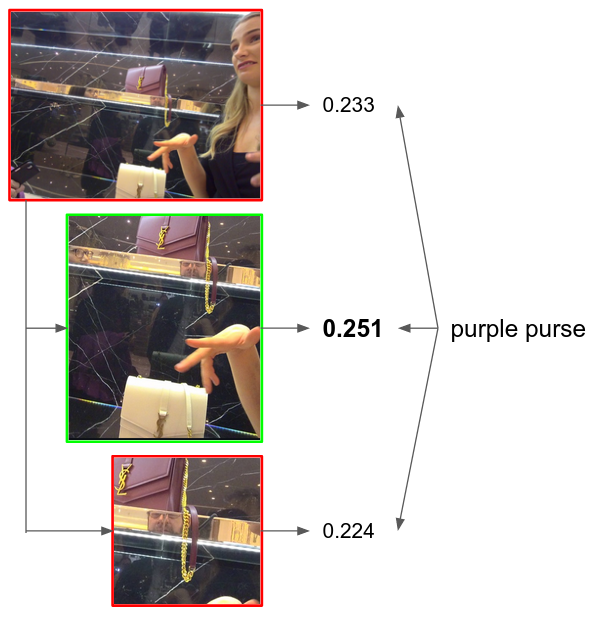
\includegraphics[width=0.7\columnwidth]{content/resources/images/methods/CaseStudy3Overview.png}
    \caption{The third scenario. The target image is shown at the top, following by a $2 \times 2$ patch and a $1 \times 1$ patch containing the purse. The images are not scaled equally. }
    \label{fig:CaseStudy3}
\end{figure}

\vspace{-2mm}
For this query, we could try to locate the shop through geolocating or finding other shopping moments and browse for a fashion shop that sells purses. We believe that there are few images of a purple purse, so we focus on this hint. However, from the description, we know that the purse does not occupy the whole image, this can make it difficult to find it if we only encode the whole image. 

Indeed, the local features mentioned in section \ref{sec:attention_based_embedding_enrichment} help us in this case, as the correct crop can better highlight the purse. Note that the varying sizes matter, as the $1 \times 1$ patches fail to capture the purse, and only the $2 \times 2$ patch is able to fully capture it. Being able to centralize on the purse while ignoring other objects pushes it closer to the "purse" concept and allows it to be found. The scenario is depicted in Figure \ref{fig:CaseStudy3}. The scores represent in the figure are the similarity (higher is better) to the query phrase "\textit{purple purse}". In this case, only the $2 \times 2$ patch is close enough to make it to the top results, the other images are too far down the ranklist. 


\subsection{Best practices}
\label{sec:best_practices}

Due to many factors, novice users (i.e., people that are not familiar with retrieval systems and/or do not have knowledge of the underlying model/data) have difficulty operating the system with performance that is comparable to expert users or system developers. In our work \citeown{hoang-xuan_flexible_nodate}, we propose to devise a few guidelines on which users can create their own strategy to use when searching. The idea for this proposal is based on the fact that in the challenges/competition, the systems are operated by developers who have a good understanding of the system, therefore they are extremely proficient when searching. The reason for this is that through extensive testing, they have become used to the scenarios that are usually presented with during the competition, and they know exactly which tools are best to overcome each obstacle. We believe this knowledge can be summed up and explained to normal users without requiring a precise understanding of the underlying system. This is especially beneficial as it dramatically improves the average performance and usefulness of the system without needing any modifications.

With all said, the compiled list of best practices is as follows:

\begin{enumerate}
    \item \textbf{Maximize specificity} \quad In a given prompt, there can be multiple concepts and objects that are being referred to. It is wise to choose the concept that is most unique to the search target since it will quickly reduce the number of possible candidates, or in terms of information theory, choose the concept that will maximize \textbf{information gain}.
    
    Example: suppose the prompt is asking for a picture of "a collection of phones, an Ipad, a wallet, and a vase on a table", it is pragmatic to look for an Ipad instead of a phone or a table. 
    
    For LSC tasks, the accompanying metadata (time, location, etc.) is especially useful here as they all help to very quickly narrow down the possible answers and should be applied almost automatically. 
    
    \item \textbf{Apply creativity} \quad More often than not, there are multiple ways to describe a single image. The differences come from word choice (simple vs advanced English), concept choice (abstract vs concrete), perception (e.g., pink vs purple), and more. Therefore, when one approach does not yield satisfactory result, it is imperative to try other avenues.
    
    Example: "a party on the beach" can also be described as "people with food on the beach", "person with plates next to sand and water", etc. 
    
    \item \textbf{Utilize visual similarity} \quad As popular search engines use text input, ordinary users are used to it. However, our system provides other means of searching as well. We emphasize the usage of visual search, as it is intuitive and easy to use yet often neglected. This feature works especially well with Ad-hoc topics. In some cases, there can be concepts that are hard to define using language, therefore an external visual example can also be used.
    
    Example: "salt lamp" is a concept that is under-represented in the data used to train the model joint-embedding model, but its visual example is sufficiently unique to search.
    
    \item \textbf{Do temporal verification} \quad People have a tendency to describe multiple moments in succession rather than a single one. This provides valuable information that can be used to distinguish the right moment from similar ones. Therefore, when dealing with multiple events, the Timeline View feature should be used to check whether the preceding/succeeding events follow the same narration. 
\end{enumerate}

\chapter{Referring Expression Segmentation}
\label{chap-refer-seg}
\begin{ChapAbstract}
In this chapter, we present our proposed method for referring expression segmentation called VLFormer. We first provide an overview of our method in Section \ref{sec:rvos_overview}. In Section \ref{sec:rvos_architecture}, we then describe our architecture in details. Our training strategy is mentioned in Section \ref{sec:rvos_training_strategy}. Then, we discuss our extended version to the video that consists of a selection strategy to choose the final object and the post-processing strategy by Semi-VOS methods for better refinement in Section \ref{sec:rvos_inference}. Section \ref{sec:rvos_ytvos} and \ref{sec:ris_dataset} present datasets we conduct the experiments and the performance of our method on those datasets. Finally, we analyse the qualitative results of our referring expression segmentation framework in Section \ref{sec:rvos_qualitative_analysis}.


\end{ChapAbstract}

\section{Overview}
\label{sec:overview}

\subsection{Introduction to Lifelog Retrieval}

In 2021, we witnessed the rising popularity of video content on platforms such as TikTok, Instagram Reels, and YouTube Shorts. Along with the promise about the metaverse, they show that content is moving from simple images to more complex forms, such as video and virtual reality. A system that can handle these new forms of data, which is more costly computational and storage-wise, can undoubtedly provide great value. While the LSC'22 dataset \cite{gurrin_introduction_2022} is not a video dataset on its own, it is similar to one, in terms of size and temporal meaning. It is greater than the previous edition (roughly 725,000 images compared to 183,299 \cite{gurrin_introduction_2021}) and poses a significant challenge to system developers \cite{gurrin_introduction_2022}.

In recent years, Transformer \cite{vaswani_attention_2017} has become the prevalent architecture in both text and image domains. They have inspired the use of large collections of unlabeled data in training, which is easier to obtain. The approach is sometimes called self-supervised learning. When large image-text or video-text datasets become available, they give rise to vision-language pre-training. This approach creates large multi-purpose image-text models pre-trained on matching images to their captions instead of performing a specific task such as classification. These models are applicable to many downstream tasks such as Video-Text Retrieval \cite{gao_clip2tv_2021}, or even zero-shot Video Retrieval \cite{portillo-quintero_straightforward_2021}. With the nature of being trained on image-text data, we believe that they are especially suitable for a cross-domain image-text retrieval task, which turns out to be exactly what LSC is.

Since the LSC competition centers around interactivity, this means that good systems also have practical value. In addition, they also hold a novice session to make sure the systems are easy to use, even for non-expert users. With that in mind, we seek to use the large vision-language pre-trained models' representational strength and versatility to empower our search engine while at the same time simplifying user interaction through a better understanding of image sequence semantics.

%Short summary about recent methods
% Providing effective access methodologies for personal lifelogs can trace its beginning back to the seminal MyLifeBits system \cite{Gemmel-2006} which indexed Gordon Bell's lifetime of digital data. To motivate and facilitate the development of more effective lifelog retrieval systems, the organizers of the Lifelog Search Challenge (LSC) launched this series of annual challenges in 2018 as a comparative benchmarking workshop with the aim of fostering scalable and effective retrieval technologies for large lifelog datasets. The LSC workshop provided participants with a large lifelog dataset and a set of topics to solve. Competing teams must find an image from the lifelog archive that best addresses the information need posed by the topic within a limited time period. In this paper, we introduce LSC'22, the fifth iteration of the Lifelog Search Challenge. %, LSC'21.

Based on FIRST 2.0 \cite{trang-trung_flexible_2021}, we revise and improve the functionalities and performance of our retrieval system, as well as integrate new components to FIRST 3.0. First, we enhance the semantic encoding for an image using CLIP \cite{radford_learning_2021}. We propose representing an image by a set of adaptive semantic embedding vectors, each corresponding to either the whole image or various regions of interest in different sizes. In this way, our system is expected to better capture the semantics of an image to search for concepts at varying levels of granularity. Second, we propose augmenting our system with an external search engine, such as Google, to find visual examples corresponding to unfamiliar concepts for our system to retrieve visually similar moments in the collection of images. Third, because of the vast amount of images, we utilize the clustering of images to shots, \textit{i.e. }sequence of contiguous similar images, and scenes, \textit{i.e.} similar shots in the same place at different time instants, to organize images in hierarchical clusters for efficient exploration.

\subsection{Introduction to Referring Expression Segmentation}
\vspace{-2mm}
Referring expression segmentation aims to predict a pixel-wise mask of the referred object given an image and a natural language expression. This task can be potentially used in a wide range of applications, including human-object interaction and image editing. Unlike traditional visual segmentation tasks (such as semantic segmentation \cite{he_adaptive_2019} and instance segmentation \cite{he_mask_2017}) that require a fixed number of categories, referring expression segmentation has to deal with a broader amount of vocabularies and syntax diversities of human languages. In this task, the target object is mentioned with various forms of expression, such as words, phrases, or complex sentences presenting the concepts of actions, positions, objects, etc. Hence, the most challenging part of this task is to understand the expression and highlight the regions that are relevant to that expression.

\vspace{-2mm}
Over the past few years, the referring expression segmentation task has grown rapidly. Early approaches \cite{liu_recurrent_2017, margffoy-tuay_dynamic_2018, li_referring_2018} leverage a fusion module between visual and linguistic features and followed by a cross-modal decoder to generate masks of the referred object. Concretely, the fusion modules includes recurrent interaction \cite{liu_recurrent_2017, li_referring_2018}, cross-modal attention \cite{shi_key-word-aware_2018, chen_see-through-text_2019}, language-guided modeling \cite{huang_referring_2020, hui_linguistic_2020}, etc. Recently, Transformer \cite{vaswani_attention_2017} shows a significant improvement in performance of cross-modal alignments \cite{ding_vision-language_2021,yang_lavt_2022, botach_end--end_2022} (illustrated in Fig. \ref{fig:comparison_pipeline}). 



\begin{figure}[!t]
    \centering
    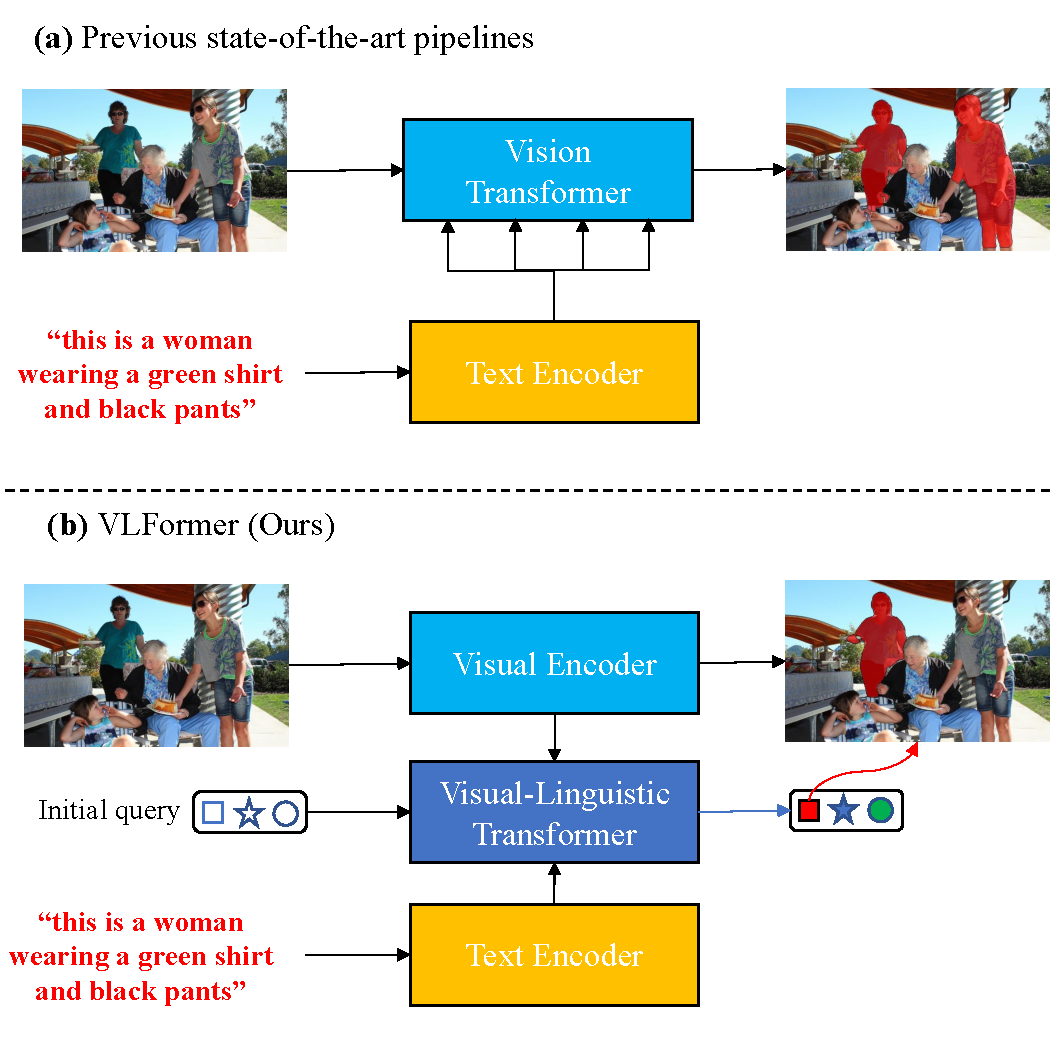
\includegraphics[width=0.7\linewidth]{content/resources/images/referring_segmentation/CompareOverview.pdf}
    \caption{Comparison of referring image segmentation pipelines. (a) The previous state-of-the-art approach (i.e., LAVT \cite{yang_lavt_2022}) integrate linguistic features into visual features of a vision transformer model to benefit the jointly exploiting vision-language cues. (b) We propose to leverage a Transformer-based module to associate both visual and linguistic information with a set of object queries, aiming to gradually update the representation of these object queries. The final object queries then produce the mask prediction.}
    \label{fig:comparison_pipeline}
\end{figure}

\vspace{-2mm}
In most previous transformer-based works in computer vision \cite{carion_end--end_2020, wang_end--end_2021, cheng_per-pixel_2021, cheng_masked-attention_2022}, a set of queries is used to represent the class or instance features for detection and segmentation. In referring segmentation task, some works \cite{ding_vision-language_2021, wu_language_2022} generate the query vectors from language features using vision-guided attention or directly. Then these queries are updated in a Transformer decoder using visual features only. It can lead to a problem that the linguistic information can vanish in the object query features after several Transformer decoder layers. To address this issue, a potential solution is to exploit a multi-modal Transformer for simultaneously aggregating visual and linguistic features during the transformer decoder.

Besides, on such referring segmentation problems, the text query usually contains information about the category, position on the image, and appearance of the object. In some cases, the related position between the referred object and others is mentioned. CLIP \cite{radford_learning_2021} models are learned from a wide range of visual concepts followed by the natural language. Hence, these models can better capture the information related to the visual concepts. 


Hence, we propose a Visual-Linguistic Transformers (VLFormer) \citeown{nguyen_vlformer_2022} approach to leverage a set of queries that understand both visual and linguistic features to represent potential objects. First, the CLIP Text Encoder is utilized for linguistic features from natural language expression. The linguistic features are used to improve the vision-language fusion and enhance the representation of object queries through the Transformer-based module. Second, a Visual-Linguistic Transformer, which contains several Visual-Linguistic Transformer Block modules, is designed for constructing fine-grained object features using linguistic and multi-scale visual information. Each Visual-Linguistic Transformer Block (VLB) utilizes the cross-attention modules from linguistic and visual features to object queries, then generates more informative object queries. Figure~\ref{fig:comparison_pipeline} highlights the difference between our proposed work and the state-of-the-art method.
\section{Architecture}
\label{sec:rvos_architecture}

\subsection{Feature Extraction}
As illustrated in Figure \ref{fig:VLFormer}, the input of our framework consists of a image $I$ and a referring expression with $L$ words. 

\textbf{Visual Encoder.}
    For an image, $I \in \mathbb{R}^{H \times W \times 3}$, we extract the multi-scale feature maps by a visual encoder. The visual encoder, e.g., ResNet, usually processes an image with five different stages that correspond to different scales: $1/2$, $1/4$, $1/8$, $1/16$, and $1/32$. 

In our model, we utilize the four last stages and transform their feature dimension into a common dimension $C$ by a Multilayer Perceptron (MLP) module for convenience. We obtain the multi-scale feature maps $\{F_v^j\} \in \mathbb{R}^{\frac{H}{2^j} \times \frac{W}{2^j} \times C}$ for each stage $j \in (2, 3, 4, 5)$, respectively.    
Note that the $H$ and $W$ are the height and width of the original image.

\textbf{Text Encoder.} 
On such referring segmentation problems, the text query usually contains the information about the category, position on the image and appearance of the object. In some cases, the related position between the referred object and others is mentioned. 

CLIP models are learned from a wide range of visual concepts followed by the natural language. Hence, these models are able to capture the information related to the visual concepts better. 

We adopt the text encoder of the CLIP ~\cite{radford_learning_2021} model to extract the linguistic features $F_t \in \mathbb{R}^{L \times C'}$ from the $L$-word expression. 
The text encoder of the CLIP model is a modified Transformer module. 
% Each word of the expression is converted into a token in a 49,252-vocab dictionary.   
For convenience in later stages (e.g., Transformer decoder), we compress the dimension $C'$ to $C$ by a MLP module so that the dimension of linguistic features is now the same as the visual features.
We also add a sinusoidal 1D positional encoding $e_{pos} \in \mathbb{R}^{L \times C} $ to the linguistic features to store the positional information in these features.

% As illustrated in Figure \ref{fig:VLFormer}, the input of our framework consists of a video $V$ and a referring expression with $L$ words. 

% \subsubsection{Visual Encoder}
% For a video with $T$ frames, $V \in \mathbb{R}^{T \times H \times W \times 3}$, we extract the multi-scale feature maps for each frame in the video independently by a visual encoder. The visual encoder (such as ResNet, SwinTransformer,...) usually extracts an image with five different stages that correspond to different scales: $1/2$, $1/4$, $1/8$, $1/16$ and $1/32$. 

% In our model, we utilize the three last stages and transform their feature dimension into a common dimension $C$ for convenience. We obtain the multi-scale feature maps $\{F^i_j\}^T_{i = 1} \in \mathbb{R}^{\frac{H}{2^j} \times \frac{W}{2^j} \times C}$ for each frame $i$ and stage $j \in (3, 4, 5)$.    
% Note that the $H$ and $W$ are the height and width of the original frame.

% \subsubsection{Text Encoder}

% On such referring segmentation problems, the text query usually contains the information about the category, position on the image and appearance of the object. In some cases, the related position between the referred object and others is mentioned. 

% CLIP models are learned from a wide range of visual concepts followed by the natural language. Hence, these models are able to capture the information related to the visual concepts better. 

% We adopt the textual encoder of the CLIP model to extract the linguistic features $F_t \in \mathbb{R}^{L \times C'}$ from the $L$-word expression. 
% The textual encoder of CLIP model is a modified Transformer module. 
% % Each word of the expression is converted into a token in a 49,252-vocab dictionary.   
% For convenience in later stages (Transformer decoder), we compress the dimension $C'$ to $C$ by a MLP module, so that the dimension of linguistic features is now the same as the visual features.


\subsection{Cross-modal Pixel Decoder}
% The multi-scale visual features that are extracted by the backbone will incorporate with the linguistics features, aiming to enrich the information related to the referred object in each frame of the video. Then will be decoded again into the fine-grained features.

% Firstly, the visual features are fused with the linguistic features ${F_t}$, extracted by the text encoder to perform an early interaction between visual and linguistic features by a Visual-Linguistic Early Fusion block (VLEF) for highlighting regions that are matched with the referring expressions. 
% \begin{equation}
%     \hat{F}_v^i = F_v^i \odot MSA(F_v^iW^Q, F_tW^K, F_tW^V)
% \end{equation}
% where MSA(q, k, v) is the multi-head attention layer and $W^Q$, $W^K$, $W_V$ $\in \mathbb{R}^{C \times d_{head}}$ are learnable parameters. This multi-head attention layer is used as a compatibility weight between the visual features and linguistic features. And then, we multiply this weight with the visual feature to focus on region high related to referring expressions. 

% The rest of Pixel Decoder is adopted from Mask2Former\cite{cheng_masked-attention_2022} with a multi-scale deformable attention module to produce a multi-scale features map  for video frames. 

The multi-scale visual features that are extracted by the visual encoder then are incorporated with the linguistics features, aiming to enrich the information related to the referred object in each frame of a video. Then will be gradually decoded again into the fine-grained features.


\begin{figure}[t]
    \centering
    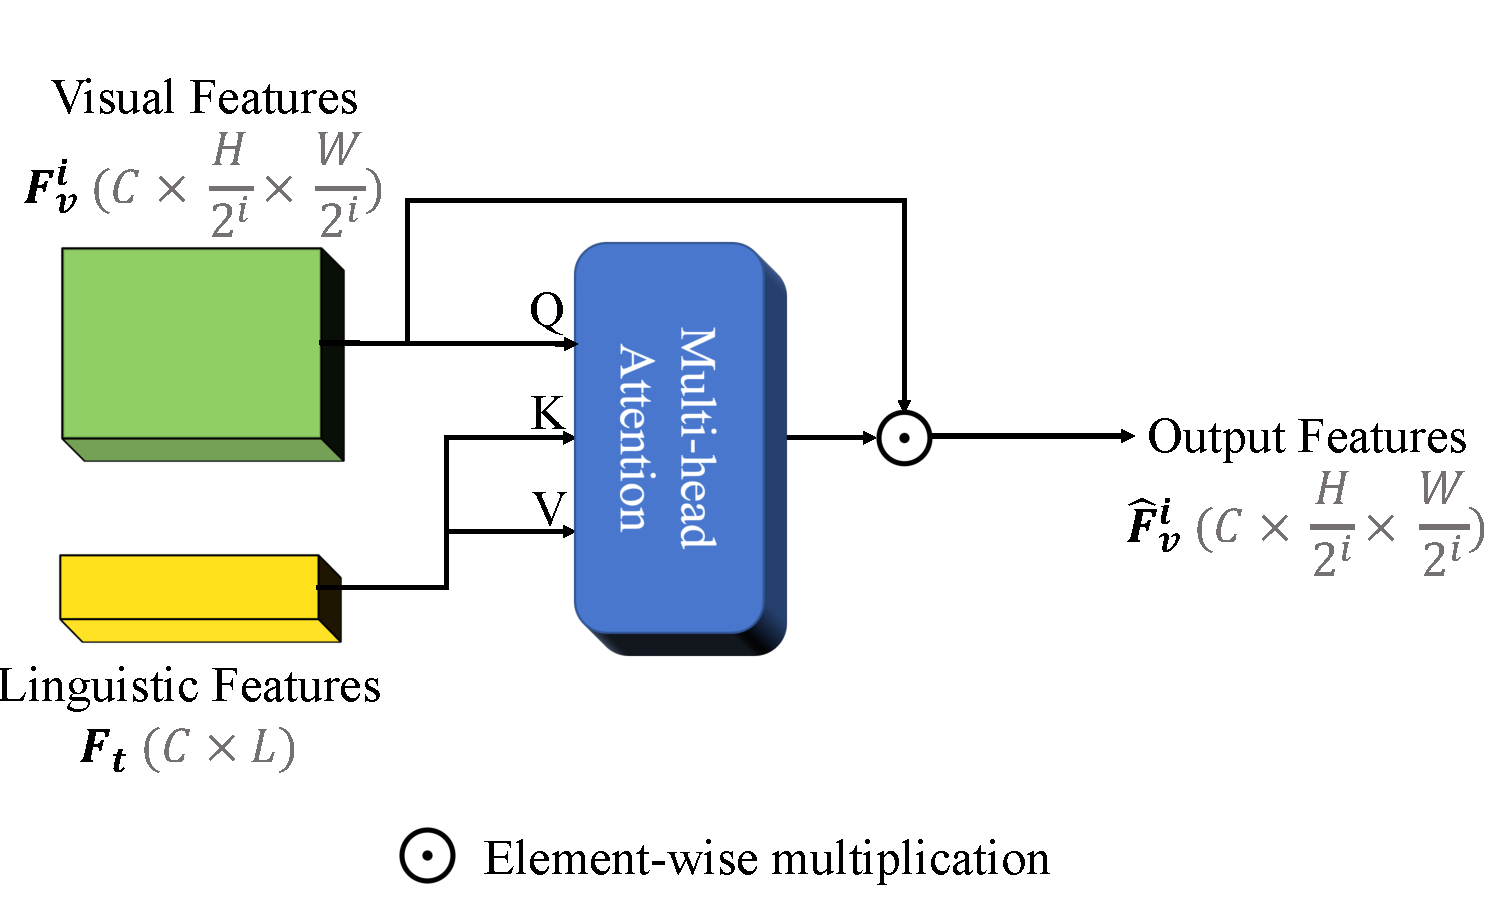
\includegraphics[width=\textwidth]{content/resources/images/referring_segmentation/Language Guidance Module.pdf}
    \caption{The implementation of Language Guidance Module. Visual features $F_v^i$ and linguistic features $F_t$ is used as input to output the language-guided visual features $\hat{F}_v^i$.}
    \label{fig:lgm}
\end{figure} 

\textbf{Language Guidance Module.} 
Firstly, the visual features are fused with the linguistic features ${F_t}$, extracted by the text encoder to perform an early interaction between visual and linguistic features by a Language Guidance Module (LGM) for highlighting regions that are matched with the referring expressions. 
\begin{equation}
    \hat{F}_v^i = F_v^i \odot MSA(F_v^iW^Q, F_tW^K, F_tW^V),
\end{equation}
where MSA(q, k, v) is the multi-head attention layer and $W^Q$, $W^K$, $W_V$ $\in \mathbb{R}^{C \times d_{head}}$ are learnable parameters. This multi-head attention layer is used as a compatibility weight between the visual features and linguistic features. Then, this weight is multiplied with the visual feature to focus on region highly related to referring expressions. Figure \ref{fig:lgm} shows the LGM implementation.


\begin{figure}[t]
    \centering
    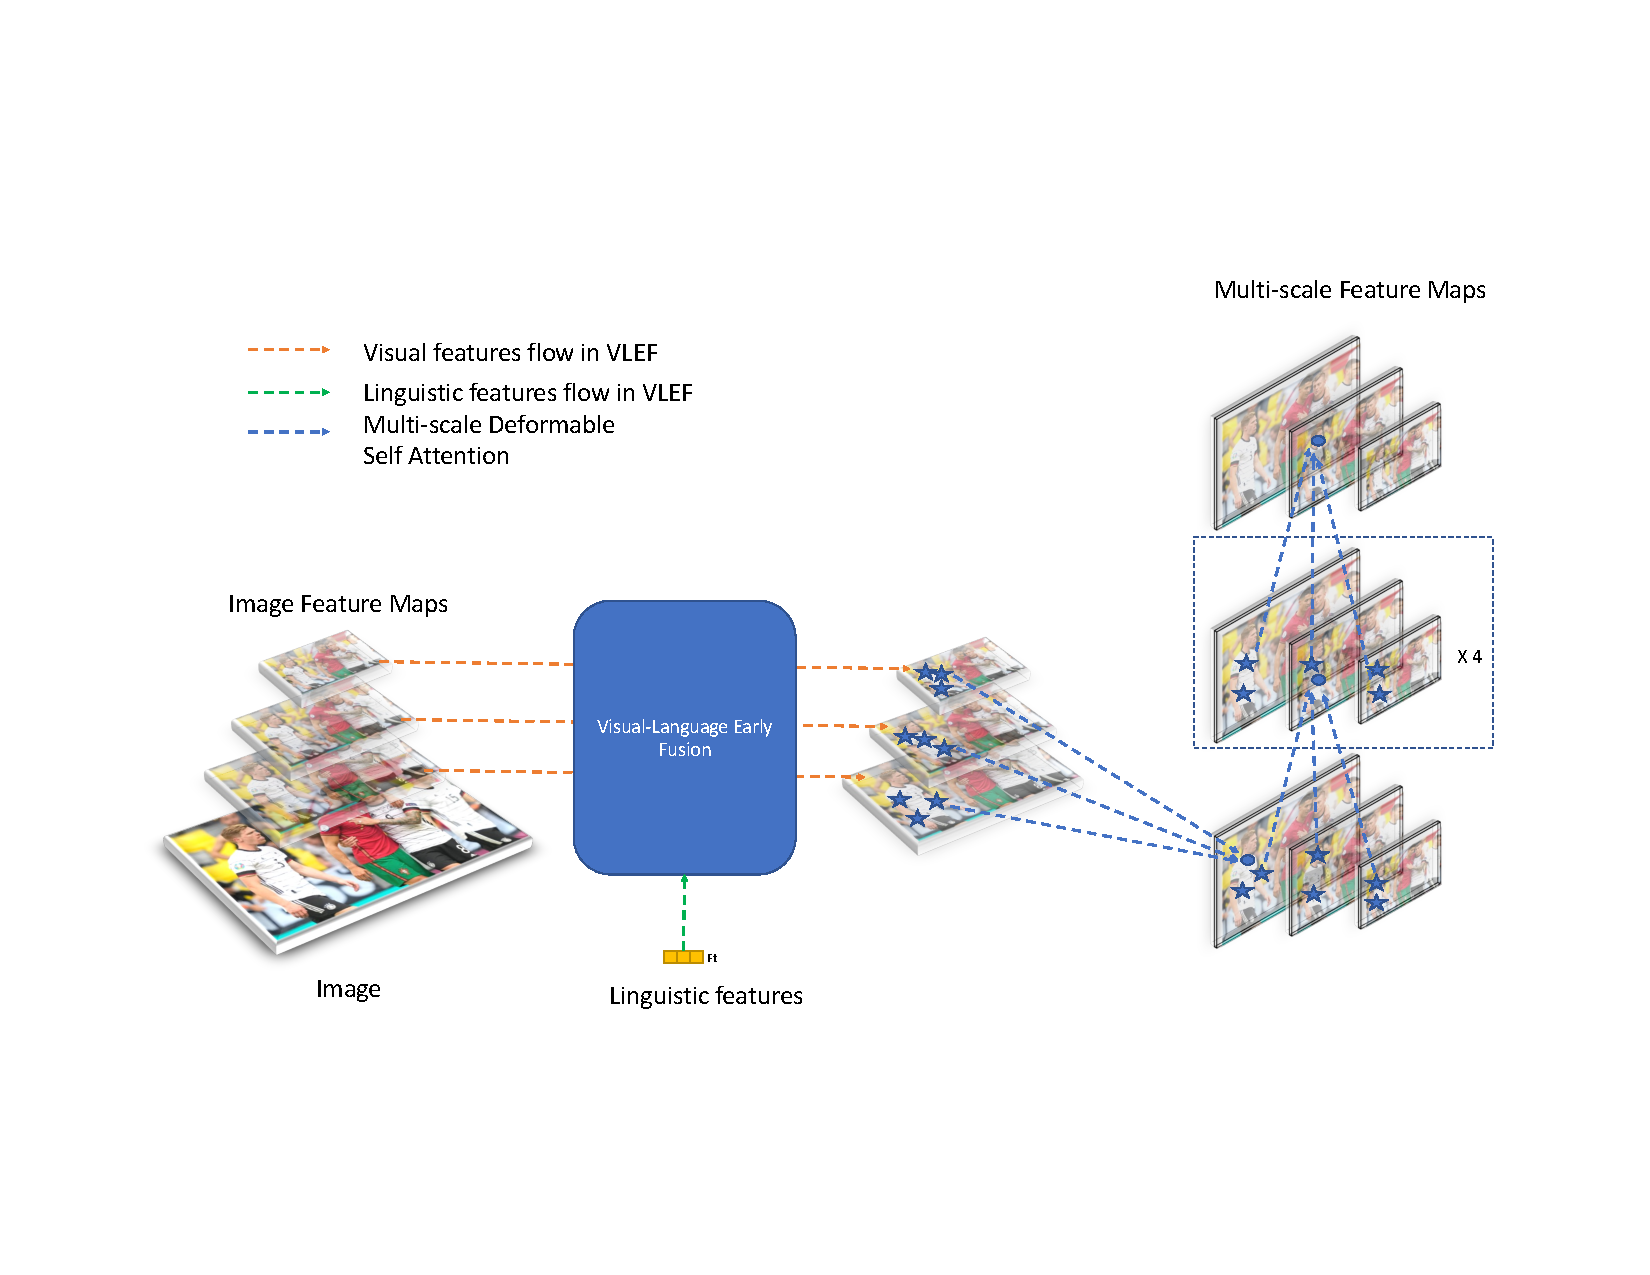
\includegraphics[width=\textwidth]{content/resources/images/referring_segmentation/Cross-modal_Pixel_Decoder.pdf}
    \caption{The overview of Cross-modal Pixel Decoder}
    \label{fig:pixel_decoder}
\end{figure}

\textbf{Pixel Decoder.}
The pixel decoder gradually upsamples the visual features $\hat{F}_v^i$ to generate the fine-grained language-guided visual features $F'_v^i$. 
The Pixel Decoder is adopted from Mask2Former \cite{cheng_masked-attention_2022} with a multi-scale deformable attention module to produce a fine-grained feature pyramid. 

\subsection{Visual-Linguistic Transformer}
\subsubsection{Visual-Linguistic Transformer Block}

\begin{figure}[ht]
    \centering
    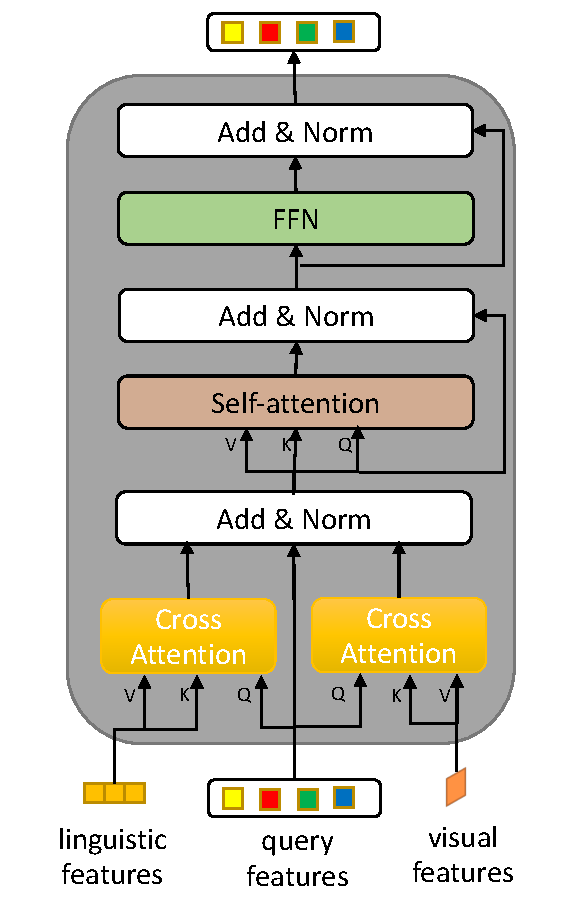
\includegraphics[width=0.5\textwidth]{content/resources/images/referring_segmentation/VLBlock.pdf}
    \caption{The architecture of Visual-Linguistic Transformer Block (VLB). The module takes query features, linguistic features $F_t$ and visual features $F'_v^i$ as input, and generates a better representation of query features.}
    \label{fig:vlb}
\end{figure}

Inspired by the Transformer decoder in Mask2Former \cite{cheng_masked-attention_2022}, we propose a Visual-Linguistic Transformer Block(VLB) to conduct the interaction between queries and visual features and between queries and linguistic features simultaneously. As illustrated in Fig. \ref{fig:vlb}, given the visual features of the video frames, linguistic features of the referring expressions, and the object queries features. 

First, the object queries interact independently with linguistic and visual features in a cross-attention way, where object queries and linguistic/visual features are query and key, respectively. 
And then, they will be summed up and fed into a multi-head self-attention module to update the object queries features and gather the contextual information of both linguistic and visual features. Finally, a FFN module is applied to these features to get the final object query features. 

\subsubsection{Multi-scale features}
Multi-scale features can help the model improve its performance, especially for various object sizes. By utilizing both low-resolution features and high-resolution features in the Transformer decoder layers, the object features can adapt with the size-changing and diversity of object's shapes. 
Specifically, we utilize the features produced by the cross-modal pixel decoder with resolutions 1/32, 1/16, and 1/8 of the original frame. 

In one Transformer decoder layer, there are 3 Visual-Linguistic Transformer blocks. In the first one, the object queries will be updated by the linguistic features and the visual features $F'_3$. In the second VLB block, The updated object queries will be re-updated by the linguistic and the visual features $F'_4$. The last VLB block updates the object queries in the same way but uses the visual feature $F'_5$ instead. 

By repeating these operations multiple times, the final object queries can be adapted with multiple-scale features and can also handle the variety of object sizes in a video. 


\subsection{Instance Matching and Loss}
\label{sec:instance_matching}
Our approach is to generate a small set of $N$ predictions, and the best one will be selected as the final object. In the training phase, therefore, we use the instance matching strategy inspired by ~\cite{cheng_masked-attention_2022, cheng_per-pixel_2021} to supervise candidate instances. 
Let us denote the prediction set as $\hat{y} = \{\hat{y_i}\}_{i = 1}^{N}$, and the prediction for the $i$-th instance is represented by:
\begin{equation}
    \hat{y}_i = \{\hat{p}_i, \hat{s}_i\}.
\end{equation}

For the $i$-th candidate instance, $\hat{p}_i \in \mathbb{R}^1$ is a probability that this instance corresponds to the referred object. Meanwhile, $\hat{s}_i \in \mathbb{R}^{H \times W}$ is the segmentation mask that we predict.

Since there is only one referred object, the ground-truth object is represented as $y \in \mathbb{R}^{H \times W}$. To train the network, we first find the best prediction $i$-th from $N$ candidates via minimizing the matching cost:

\begin{equation}
\begin{split}
    \mathcal{L}_{match}(y, \hat{y}_i) = \gamma_{cls}\mathcal{L}_{cls}(\hat{p}_i, 1) + \gamma_{mask}\mathcal{L}_{mask}(\hat{s}_i, y) \\ + \gamma_{dice}\mathcal{L}_{dice}(\hat{s}_i, y).
\end{split}
\end{equation}
The matching cost is computed based on three loss functions. First, $\mathcal{L}_{cls}$ represents the loss function for the probability a query is the referred object, and we use the Cross-Entropy loss in this work. Second, $\mathcal{L}_{mask}$ is the cross entropy loss that is designed to supervise the mask prediction. Finally, the $\mathcal{L}_{dice}$ is added to improve the dice score, which is quite similar to the IoU metric. 
$\gamma_{cls}, \gamma_{mask}$ and $\gamma_{dice}$ are the coefficients of the three corresponding losses. 

Our goal is to minimize the $\mathcal{L}_{match}$ of one query and maximize the probability of other queries $\hat{p}_j (j \not= i) $ approximate zero (it means these queries do not represent for the referred object). Therefore, our loss function is described as follows: 
\begin{equation}
    \mathcal{L}(y, \hat{y}, i) = \mathcal{L}_{match}(y, \hat{y}_i) + \sum_{\substack{j = 1 \\ j \not=i}}^{N}{\gamma_{cls}\mathcal{L}_{cls}(\hat{p}_j, 0).}
\end{equation}

% \subsection{Instance Sequence Matching and Loss}

% Our approach is to generate the set of $N$ predictions for each frame in $T$ frames. And the $i$-th prediction in all $T$ frames is to track and segment the same object, which is mentioned in \cite{wu_language_2022,cheng_masked-attention_2022}. We can maintain the same relative positions due to sharing object queries between frames. Therefore, we can easily supervise the instance sequence using the instance matching strategy followed \cite{cheng_masked-attention_2022, cheng_per-pixel_2021}. 
% Let us denote the prediction set as $\hat{y} = \{\hat{y_i}_{i = 1}^{N}\}$, and the prediction for the $i$-th instance is represented by:
% \begin{equation}
%     \hat{y}_i = \{\hat{p}_i^t, \hat{s}_i^t\}_{i = 1}^T
% \end{equation}

% For the $t$-th frame, $\hat{p}_i^t \in \mathbb{R}^1$ is a probability that this instance corresponds to the referred object or not. And $\hat{s}_i^t \in \mathbb{R}^{H \times W}$ is the segmentation mask that we predict.

% Since there is only one referred object in the video, the ground-truth instance sequence is represented as $y = \{s^t\}_{t = 1}^T$. To train the network, we first find the best prediction $i$-th from $N$ candidates via minimizing the matching cost:

% % \usepackage{amsmath}
% % \DeclareMathOperator*{\argmax}{arg\,max}
% % \DeclareMathOperator*{\argmin}{arg\,min}

% \begin{equation}
%     \mathcal{L}_{match}(y, \hat{y}_i) = \gamma_{cls}\mathcal{L}_{cls}(\hat{p}_i^t, 1) + \gamma_{mask}\mathcal{L}_{mask}(s_i^t, \hat{s}_i^t) + \gamma_{dice}\mathcal{L}_{dice}(s_i^t, \hat{s}_i^t)
% \end{equation}
% $\mathcal{L}_{cls}$ represents the loss function for the probability a query is the referred object and we use the Cross Entropy loss in this work. $\mathcal{L}_{mask}$ is the binary focal loss that is designed to supervise the mask prediction. And the $\mathcal{L}_{dice}$ is added to improve the dice score, which is quite similar to the IoU metric.
% $\gamma_{cls}, \gamma_{mask}$ and $\gamma_{dice}$ are the coefficients of corresponding losses. 


% Our goal is to minimize the $\mathcal{L}_{macth}$ of one query and the probabilities of other queries $\hat{p}_j (j \not= i) $ approximate zero (it means these queries do not represent for the referred object). Therefore, our loss function is described as follows: 
% \begin{equation}
%     \mathcal{L}(y, \hat{y}, i) = \mathcal{L}_{match}(y, \hat{y}_i) + \sum_{\substack{j = 1 \\ j \not=i}}^{N}{\gamma_{cls}\mathcal{L}_{cls}(\hat{p}_j^t, 0)}
% \end{equation}
\section{Training strategy}
\label{sec:rvos_training_strategy}
\subsection{Deep supervision}
Training a deep neural network is challenging. Due to the vanishing gradient problem, the final loss may not be effectively back propagated to the shallow layers. To address this issue, we add more auxiliary losses after each Visual-Linguistic Transformer Block.

Specifically, when the object queries are updated, these features will be multiplied with the pixel-level embeddings of the pixel decoder to generate the probability segmentation map. By utilizing the same loss function for this segmentation map, we can obtain the auxiliary loss at this stage. Without these losses, the model's target is to create a final object features represented by the referred object and the outputs of previous blocks are not paid attention to. Then those outputs can be anything, and we could not handle them. With auxiliary losses, however, the model can learn robust features even in the early layers. Then the deeper blocks the object queries are fed into, the more accurate they are. 


\subsection{Efficient training memory}
% Describe how to reduce the mem, time, and cost when using PointRend strategy to calculate the loss. 

Due to the lacking resources for training, especially in GPU VRAM, reducing the size of the model used to be the only way. Thanks to PointRend, Implicit PointRend, and Mask2Former, we can now build a larger model with small memory. The research shows that training the mask loss on $K$ randomly sampled points instead of the whole mask reduces not only the usage memory but also improves the performance. 
We choose $K = 112 \times 112 = 12544$, the memory used is decreasing dramatically, and it helps us save a lot of resources to train the network.








% \section{Inference}
% \label{sec:rvos_inference}
\section{An extension of Referring Video Object Segmentation}
\label{sec:rvos_inference}
Given a video clip $V = \{V_1, V_2, ..., V_T\}$ and a referring expression with $L$ words. Our approach is to generate the set of $N$ predictions for each frame in $T$ frames. And the $i$-th prediction in all $T$ frames is to track and segment the same object. We can maintain the same relative positions due to our efficient architecture design of sharing object queries between frames.

% \subsection{Instance Sequence Matching and Loss}
% Our approach is to generate the set of $N$ predictions for each frame in $T$ frames. And the $i$-th prediction in all $T$ frames is to track and segment the same object. We can maintain the same relative positions due to sharing object queries between frames.

% Let us denote the prediction set as $\hat{y} = \{\hat{y_i}_{i = 1}^{N}\}$, and the prediction for the $i$-th instance is represented by:
% \begin{equation}
%     \hat{y}_i = \{\hat{p}_i^t, \hat{s}_i^t\}_{i = 1}^T
% \end{equation}

% For the $t$-th frame, $\hat{p}_i^t \in \mathbb{R}^1$ is a probability that this instance corresponds to the referred object or not. And $\hat{s}_i^t \in \mathbb{R}^{H \times W}$ is the segmentation mask that we predict.

% Since there is only one referred object in the video, the ground-truth instance sequence is represented as $y = \{s^t\}_{t = 1}^T$. To train the network, we first find the best prediction $i$-th from $N$ candidates via minimizing the matching cost:

% % % \usepackage{amsmath}
% % % \DeclareMathOperator*{\argmax}{arg\,max}
% % % \DeclareMathOperator*{\argmin}{arg\,min}

% \begin{equation}
%     \mathcal{L}_{match}(y, \hat{y}_i) = \gamma_{cls}\mathcal{L}_{cls}(\hat{p}_i^t, 1) + \gamma_{mask}\mathcal{L}_{mask}(s_i^t, \hat{s}_i^t) + \gamma_{dice}\mathcal{L}_{dice}(s_i^t, \hat{s}_i^t)
% \end{equation}

% % $\mathcal{L}_{cls}$ represents the loss function for the probability a query is the referred object and we use the Cross Entropy loss in this work. $\mathcal{L}_{mask}$ is the binary focal loss that is designed to supervise the mask prediction. And the $\mathcal{L}_{dice}$ is added to improve the dice score, which is quite similar to the IoU metric.
% % $\gamma_{cls}, \gamma_{mask}$ and $\gamma_{dice}$ are the coefficients of corresponding losses. 


% Our goal is to minimize the $\mathcal{L}_{macth}$ of one query and the probabilities of other queries $\hat{p}_j (j \not= i) $ approximate zero (it means these queries do not represent for the referred object). Therefore, our loss function is described as follows: 
% \begin{equation}
%     \mathcal{L}(y, \hat{y}, i) = \mathcal{L}_{match}(y, \hat{y}_i) + \sum_{\substack{j = 1 \\ j \not=i}}^{N}{\gamma_{cls}\mathcal{L}_{cls}(\hat{p}_j^t, 0)}
% \end{equation}

\subsection{Selection strategy}

After performing a multiplication between the final object queries and the pixel-level embeddings from the pixel decoder, we obtain the probability segmentation map for $N$ candidate instances $S \in \mathbb{R}^{N \times T \times H \times W}$
Among $N$ candidates, we need a strategy to choose the correct one. Our strategy is to use the predicted probabilities to generate the confidence score for each candidate in the whole video. We obtain the confidence score set $P_i = \{p_{i}\}^N_{j = 1}$ by averaging the predicted probabilities over all the frames for each instance query. We select the instance with the highest score, and its index is donated as $\sigma$. 

The segmentation mask for each frame is obtained from the mask candidates set by selecting the corresponding query index $\sigma$. 

\subsection{Post-processing}
The prediction is not always segmented smoothly and continuously in case there are several objects that are similar to the referred object. To deal with this, semi-supervised Video Object Segmentation(Semi-VOS) methods can handle the problem. Semi-VOS aims to segment objects given the ground truth of them for the first frame.   

Regarding our problem, there is no ground-truth mask for any frames in the inference. However, after predicting the whole video, we have already had the preliminary results, and we can leverage these predictions to refine the target masks by using a Semi-VOS method. STCN is the state-of-the-art in the Semi-VOS tasks by constructing a memory bank of several pair frames and their annotations and utilizing the information from that bank to segment the corresponding objects in the query frame. 

We do not have any actual ground truth, which means we can not identify which object in which frame is the correct one to reference. We assume that most of the frames are referred to the correct one, and our goal is to refine the boundary and re-identify the target object in the rest of the video. Hopefully, STCN is the best candidate to carry out our goal. Our strategy is described as follows.

First, we uniformly sample K = 10 keyframes for each video sequence.
% The more keyframes we used, the more resources we consume to predict a query frame. Moreover,  
Then, these keyframes and their corresponding masks are memorized in a memory bank of the STCN\cite{cheng_rethinking_2021}. 
Finally, we re-predict the whole video by STCN and update the memory bank every 5 frames. 
\section{YouTube-VOS Challenge 2022}
\label{sec:rvos_ytvos}
The YouTube-VOS Challenge provides a large-scale dataset for video object segmentation tasks, allowing us to design an algorithm to solve the long-term spatial-temporal dependency explicitly. Since 2018, it has been organized every year except the year of 2020. The challenge has introduced three challenges for different video object segmentation tasks, including:
\begin{itemize}
    \item Semi-supervised Video Object Segmentation
    \item Video Instance Segmentation
    \item Referring Video Object Segmentation
\end{itemize}

In 2022, The 4th Large-scale Video Object Segmentation Challenge was held as a workshop in conjunction with CVPR 2022, New Orleans, Lousiana. In the Video instance segmentation tasks, there is an extend of long video for validation and testing. 
% We participated in the Track 3: Referring Video Object Segmentation to experiment our method 

\subsection{Dataset}
The dataset was created based on the YouTube-VOS-2019 dataset, called Refer-YouTube-VOS. 
The Refer-Youtube-VOS contains 3,978 high-resolution YouTube videos with 131k high-quality manual annotations and 15k language expressions. The dataset is divided into 3,471 training videos, 202 validation videos, and 305 test videos.

\subsection{Evaluation metrics}
The region similarity($\mathcal{J}$) and contour accuracy($\mathcal{F}$) are used as the evaluation metrics for this challenge. The final ranking is sorted according to the average between these two metrics. 
\label{sec:metric}
\begin{itemize}
    \item \textbf{Region similarity $\mathcal{J}$} - To measure the similarity of region-based segmentation, i.e., the number of correct pixels and mislabeled pixels, the Jaccard index $\mathcal{J}$ is used. The Jaccard index, also known as the IoU metric, is to quantify the percent overlap between the target mask and our prediction. For simplification, the Jaccard index can be calculated by the division of the number of common pixels between the target mask and the prediction over the total number of pixels appearing across both masks. Given an output segmentation $P$ and the ground-truth mask $G$, it is defined as  

\begin{equation}
    \mathcal{J} = \frac{|P \cap G|}{|P \cup G|}
\end{equation}

with $|X|$ is the area of that segmentation. 
    \item \textbf{ Contour accuracy $\mathcal{F}$} - From a contour-based perspective, we can consider a segmentation $P$ as a set of closed contours $c(P)$ which delimits the spatial extent of the mask. We can compute the contour-based precision $P_c$ and recall $R_c$ between the contour points $c(P)$ and $c(G)$ of the output segmentation and ground-truth, respectively, via a bipartite graph matching in order to maximize the accuracies. The F-measure $\mathcal{F}$ is used as a good trade-off between precision and recall, defined as 
\begin{equation}
    \mathcal{F} = \frac{2P_c R_c}{P_c + R_c}
\end{equation}
\end{itemize}

\subsection{Implementation details}
We used Detectron2 to train our network. The text encoder is frozen during the training stage. In the Transformer Decoder, we choose L = 2 with 6 decoder layers in total. The initial backbone weights have been previously pretrained on YouTube-VIS 2021 from Mask2Former \cite{cheng_masked-attention_2022}. STCN is pretrained mainly on saliency datasets and finetuned over training splits of semi-supervised VOS tasks.
We train the network for 100k iterations using the AdamW optimizer with the initial learning rate $10^{−4}$. A factor of 0.1 decreases the learning rate at the $70.000$-th iteration. We train the network with a small batch size of 2 on 2 Tesla V100 with 16GB GPU.

\subsection{Results}


\begin{table}[ht]
    \centering
    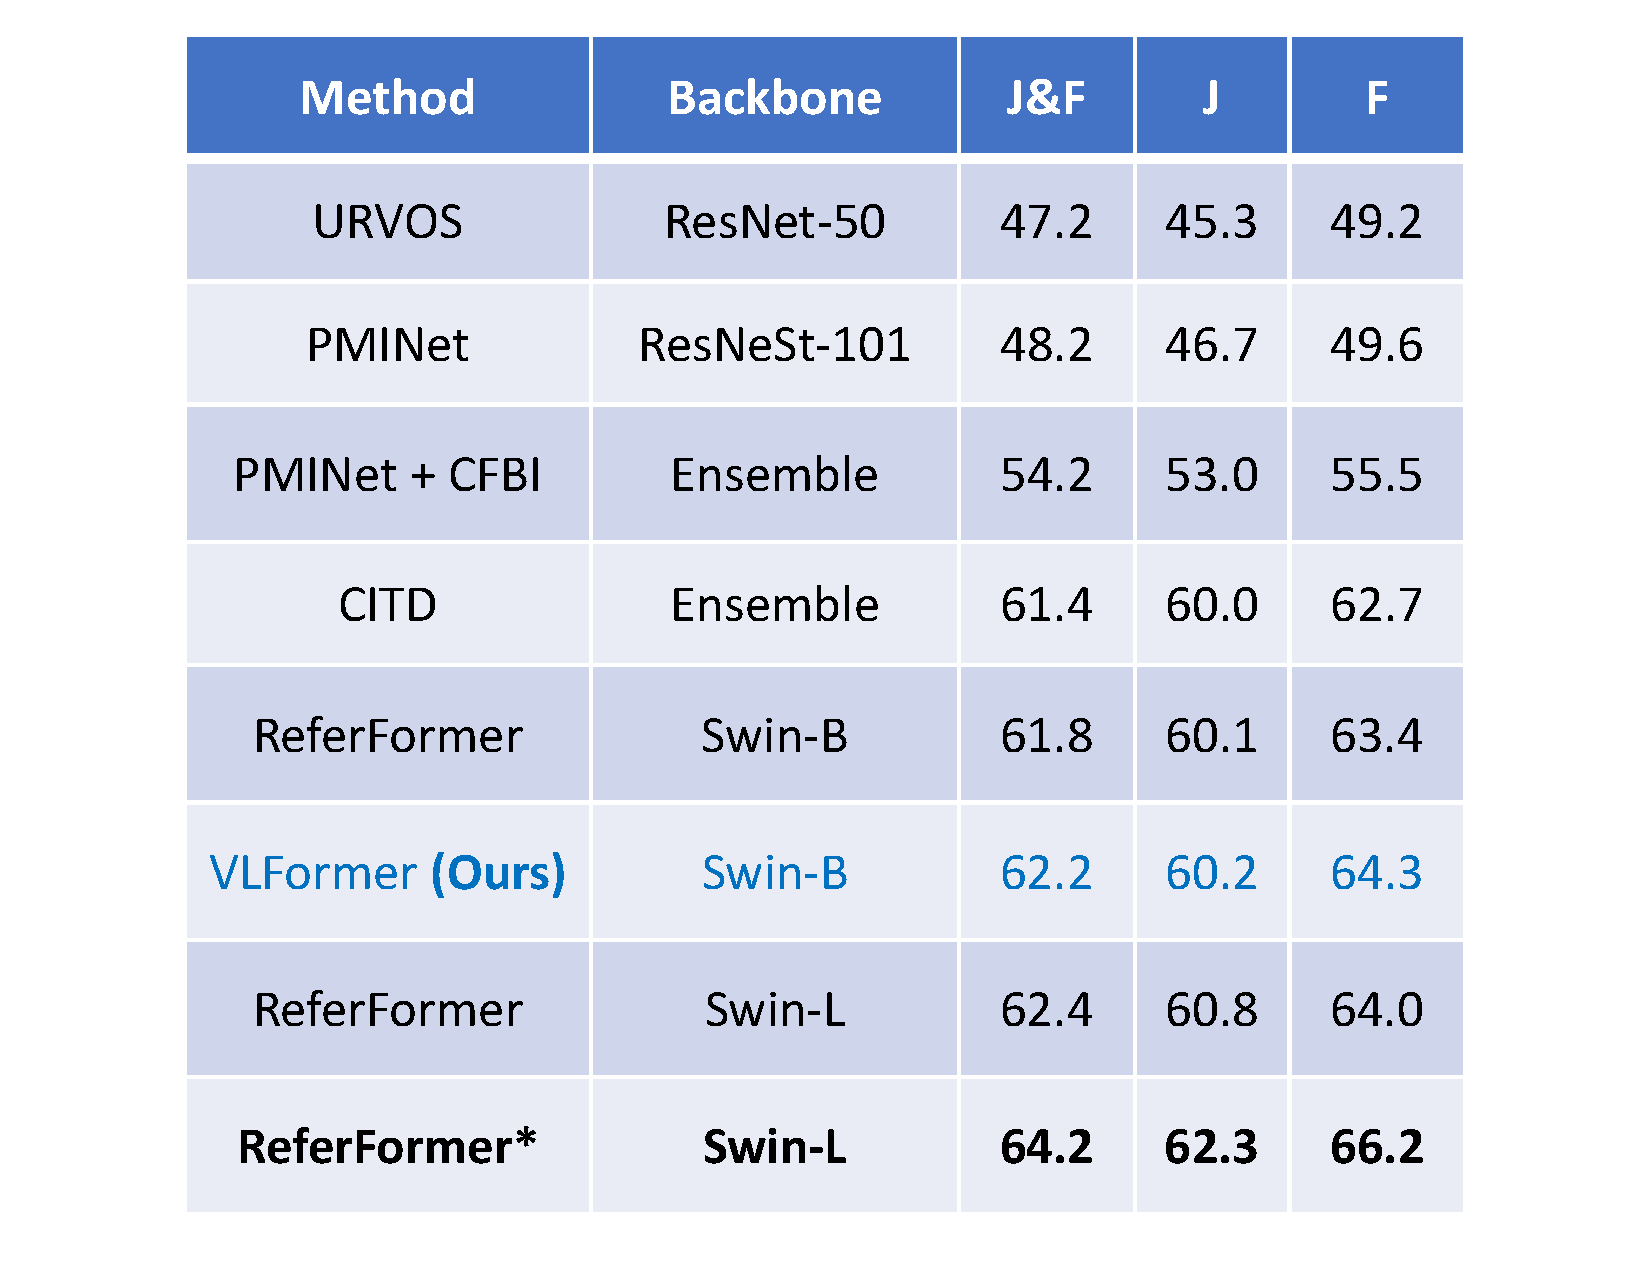
\includegraphics[width=\textwidth]{content/resources/images/referring_segmentation/RefYoutubeVOS2022-SOTA.pdf}
    \caption{Comparison with the state-of-the-art methods on Refer-Youtube-VOS development dataset. * means joint training with external datasets.}
    \label{tab:refyoutube2022_dev}
\end{table}


\begin{table}
\centering
% \resizebox{\linewidth}{!}{ %< auto-adjusts font size to fill line
\begin{tabular}{@{}clccc@{}}
\toprule
 & Team & $\mathcal{J\&F}(\uparrow)$ & $\mathcal{J}(\uparrow)$ & $\mathcal{F}(\uparrow)$ \\
\midrule
1 & Bo\_\_\_ & 0.641 & 0.622 & 0.661 \\
2 & jiliushi & 0.617 & 0.598 & 0.636 \\
3 & PENG & 0.608 & 0.589 & 0.627 \\
4 & ds-hohhot & 0.596 & 0.579 & 0.612 \\
5 & JQK & 0.594 & 0.577 & 0.611 \\
6 & nero(\textbf{Ours}) & 0.580 & 0.561 & 0.599\\
\bottomrule
\end{tabular}
% } % \resizebox
\caption{
% 
Results in Ref-YouTube-VOS 2022 \textit{test} set.
% 
} % \caption
\label{tab:refyoutube2022}
\end{table}

Table \ref{tab:refyoutube2022_dev} shows our results in the Refer-Youtube-VOS 2021 development set. The table also shows the comparison between our approach and state-of-the-art methods in the same datasets. Our approach achieves 62.2\% in overall ($\mathcal{J\&F}$) with 60.2\% and $64.3\%$ in $\mathcal{J}$ and $\mathcal{F}$, respectively. As we can see, we can surpass the previous competitive method with an ensemble technique and post-processing as PMINet + CFBI, CITD\cite{liang_rethinking_nodate} with a considerable margin of 8\% and 0.8\%. Compared to the current state-of-the-art ReferFormer\cite{wu_language_2022}, in the same backbone Swin-B, we slightly beat ReferFormer of 0.4\%. A larger backbone Swin-L in ReferFormer achieves just 62.4\% compared to 62.2\% of ours, and after joint training with external datasets, the results of ReferFormer Swin-L increase 1.8\% (from 62.4\% to 64.2\%) in overall. However, our method is still promising. Due to the lack of resources, we can not train our method with the same computational system as ReferFormer. We used only two 12GB VRAM RTX 2080 Ti instead of 8-16 NVIDIA Tesla V100 (32GB VRAM) as ReferFormer. 

Table \ref{tab:refyoutube2022} shows the leaderboard of the YouTubeVOS Challenge 2022 Track 3: Referring Video Object Segmentation on the testing set. The top 5 teams focused on heavy inference and post-processing, such as: Inference with multiple scales, multiple augmentations (flip horizontal, vertical,...), and multiple semi-supervised video object segmentation models for post-processing. Meanwhile, our team \citeown{nguyen_visual-language_2022} ranks 6th without just only one scale in inference and post-processing. No ensemble technique is used in our method.

\section{RefCOCO, RefCOCO+ and G-Ref}
\label{sec:ris_dataset}
\subsection{Dataset}
% The datasets were collected using the ReferitGame. In this two-player game, the first player is given an image with a segmented object and asked to write a language expression to describe the target object. The second one is shown only the image and the referring expression and asks to choose the corresponding object. 
% RefCOCO has 142,209 expressions for 50,000 objects in 19,994 images, and RefCOCO+ consists of 141,564 expressions for 49,856 objects in 19,992 images. 

We evaluate our VLFormer on three commonly used datasets for referring image segmentation: RefCOCO, RefCOCO+ and G-Ref.

\textbf{RefCOCO \& RefCOCO+} were collected using the two-player  ReferitGame. In this game, the first player is given an image with a segmented object and asked to write a language expression to describe the target object. The second one is shown only the image and the referring expression and asks to choose the corresponding object. 
RefCOCO has 142,209 expressions for 50,000 objects in 19,994 images, and RefCOCO+ consists of 141,564 expressions for 49,856 objects in 19,992 images. Some kinds of words, e.g., words about absolute locations, are not used in the RefCOCO+ dataset. Therefore, it is considered to be more challenging than the RefCOCO dataset. The expressions in RefCOCO and RefCOCO+ are very concise, contains 3.5 words on average, and tend to have more objects of the same category per image (3.9 on average).

\textbf{G-Ref} is another commonly widely used dataset. It contains 104,560 expressions referring to 54,822 objects belonging to 26,711 images. Compared to RefCOCO and RefCOCO+, the average sentence length in G-Ref dataset is longer (8.4 words on average), and G-Ref has a richer word usage. However, G-Ref has fewer objects of the same category per image than RefCOCO and RefCOCO+ (1.6 on average).

\subsection{Evaluation metrics}
There are two metrics we use for experiments: IoU and Precision@X. The IoU score shows the quality of the prediction overlapped with the ground-truth, which demonstrates the overall performance of the approach. The detail of this metric is described in the section \ref{sec:metric}. The Precision@X reports the successful referring rate at the threshold X of the IoU score, which focuses on the referring ability of the method.

% The common evaluation metric used in the RefCOCO and RefCOCO+ is the IoU score. The detail of this metric is described in the section \ref{sec:metric} 

% \subsection{Results}
\subsection{Comparison with State-of-the-art}

% \begin{table}[ht]
%     \centering
%     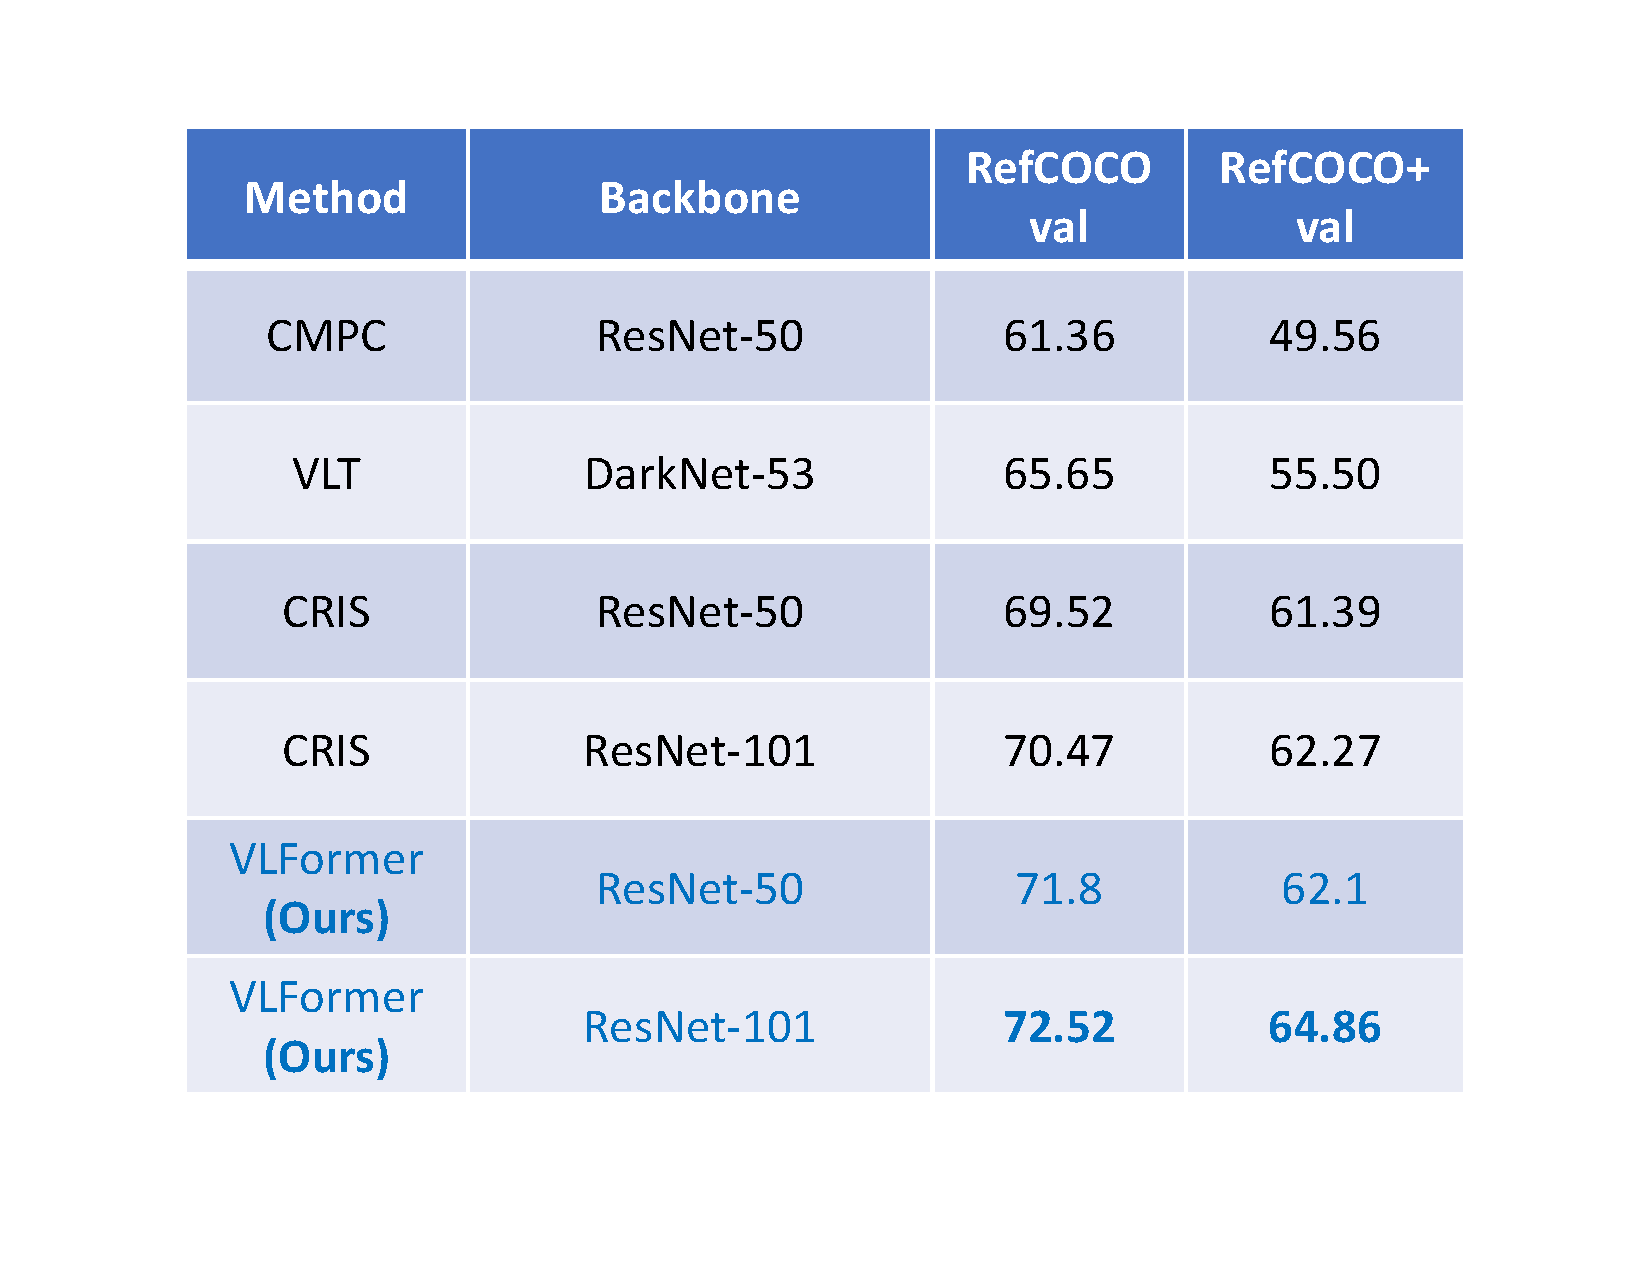
\includegraphics[width=\textwidth]{content/resources/images/referring_segmentation/RefCOCO-SOTA.pdf}
%     \caption{Comparison with the state-of-the-art methods on RefCOCO dataset.}
%     \label{tab:refcoco}
% \end{table}

 
\begin{table*}[ht]
\centering
\begin{tabular}{c|c|ccc|ccc}
\toprule

\multirow{2}{*}{Method} & \multirow{2}{*}{Backbone} & \multicolumn{3}{c|}{RefCOCO} & \multicolumn{3}{c}{RefCOCO+} \\ \cline{3-8} 
                        &                           & val      & testA   & testB   & val      & testA    & testB      \\ \midrule
MAttNet~\cite{yu_mattnet_2018}                    & ResNet-101                & 56.51    & 62.37   & 51.70   & 46.67    & 52.39    & 40.08          \\
NMTree~\cite{liu_learning_2019}                    & ResNet-101                & 56.59    & 63.02   & 52.06   & 47.40    & 53.01    & 41.56          \\
CMSA~\cite{ye_cross-modal_2019}                    & ResNet-101                & 58.32    & 60.61   & 55.09   & 43.76    & 47.60    & 37.89           \\
Lang2Seg~\cite{chen_referring_2019}                    & ResNet-101                & 58.90    & 61.77   & 53.81   & -    & -    & -            \\
CMPC~\cite{huang_referring_2020} & ResNet-101                & 61.36    & 64.53   & 59.64   & 49.56    & 53.44    & 43.23          \\
EFNet~\cite{feng_encoder_2021}                    & ResNet-101                & 62.76    & 65.69   & 59.67   & 51.50    & 55.24    & 43.01         \\
VLT~\cite{ding_vision-language_2021}                     & DarkNet-53                & 65.65    & 68.29   & 62.73   & 55.5     & 59.2     & 49.36     \\
ReSTR~\cite{kim_restr_2022}                   & ViT-B-16                  & 67.22    & 69.3    & 64.45   & 55.78    & 60.44    & 48.27       \\
CRIS~\cite{wang_cris_2022}                    & ResNet-101                & 70.47    & 73.18   & 66.1    & 62.27    & 68.08    & 53.68    \\
LAVT~\cite{yang_lavt_2022}                    & Swin-B                    & 72.73    & 75.82   & 68.79   & 62.14    & 68.38    & 55.1        \\ \midrule
VLFormer\textbf{(Ours)}                    & ResNet-50                    & 73.92    & 76.03   & \textbf{70.86}   & 64.02    & 69.74    & 55.04        \\ 
VLFormer\textbf{(Ours)}                     & ResNet-101                & \textbf{74.67}    & \textbf{76.8}    & 70.42   & \textbf{64.80}    & \textbf{70.33}    & \textbf{56.33}       \\
\bottomrule
\end{tabular}


\caption{Comparisons with the state-of-the-art approaches on RefCOCO and RefCOCO+ benchmarks. We report the results of our method with various visual backbones. IoU is used as the main metric, and  ``-'' shows that the result is not available. The best performance is marked in boldface.}
\label{tab:sota}
\end{table*}


\begin{table*}[ht]
\centering
\begin{tabular}{c|c|cc}
\toprule

\multirow{2}{*}{Method} & \multirow{2}{*}{Backbone} & \multicolumn{2}{c}{G-Ref} \\ \cline{3-4} 
                        &                           & val         & test        \\ \midrule
MAttNet~\cite{yu_mattnet_2018}                    & ResNet-101                   & 47.64           & 48.61          \\
NMTree~\cite{liu_learning_2019}                    & ResNet-101                & 46.59           & 47.88           \\
Lang2Seg~\cite{chen_referring_2019}                    & ResNet-101                  & 46.37           & 46.95           \\

VLT~\cite{ding_vision-language_2021}                     & DarkNet-53                 & 52.99       & 56.65       \\
ReSTR~\cite{kim_restr_2022}                   & ViT-B-16                    & 54.48       & -           \\
CRIS~\cite{wang_cris_2022}                    & ResNet-101                 & 59.87       & 60.36       \\
LAVT~\cite{yang_lavt_2022}                    & Swin-B                     & 61.24       & 62.09       \\ \midrule
VLFormer\textbf{(Ours)}                    & ResNet-50                    & 65.69       & 65.90       \\ 
VLFormer\textbf{(Ours)}                     & ResNet-101 & \textbf{66.77}       & \textbf{66.52}       \\
\bottomrule
\end{tabular}


\caption{Comparisons with the state-of-the-art approaches on G-Ref dataset. We report the results of our method with various visual backbones. IoU is used as the main metric, and  ``-'' shows that the result is not available. The best performance is marked in boldface.}
\label{tab:sota2}
\end{table*}
% We compare our proposed method, VLFormer, with several state-of-the-art methods on two commonly used datasets: RefCOCO and RefCOCO+. As illustrated in Table \ref{tab:refcoco}, our method surpasses other methods on all datasets even though we utilize the ResNet-50. 

% On the RefCOCO and RefCOCO+, our model with ResNet-101 backbone significant outperforms the state-of-the-art CRIS\cite{wang_cris_2022} by 2.05\% and 2.59\%, respectively. It shows that our VLFormer performs an impressive ability to gather cross-model information to perfectly segmenting the target object.   

% Our approach and Vision-Language Transformer(VLT)\cite{ding_vision-language_2021} also rely on Transformer, however a huge gap between our approach and VLT with around 7\% and 9\% for RefCOCO and RefCOCO+, respectively, which indicates that our model effectively utilizes the knowledge of CLIP Text Encoder and the query-based mechanism. 


We compare our proposed method with several state-of-the-art methods on three common datasets for referring image segmentation. As illustrated in Table \ref{tab:sota}, our method suppresses other methods on each split of all datasets with large margins. The experiments demonstrate our method can surpass the state-of-the-art in several split of datasets even though we leverage the ResNet-50 visual backbone\cite{he_deep_2016}. 

On the RefCOCO dataset, our model significant outperforms the state-of-the-art LAVT\cite{yang_lavt_2022} by 1.94\%, 0.98\% and 1.63\% on three splits, respectively even our ResNet-101 visual backbone instead of SwinTransformer-Base. 

Similarly, VLFormer achieves impressive performance gains of around 2\% than several state-of-the-art methods on each split of the more challenging RefCOCO+ dataset.

Besides, on the most challenging dataset G-Ref, which has longer and more complex expressions, our proposed VLFormer outperforms the previous state-of-the-art with wide margins of 4.97\% and 4.43\% on the validation and test subsets, respectively. As shown in Table \ref{tab:sota2}, the results demonstrate that our proposed approach has the powerful ability to understand long and complex sentences. 






\subsection{Implementation details}
% In the RefCOCO and RefCOCO+ dataset, we train the network for $10$ epochs using the AdamW optimizer with the initial learning rate $10^{−4}$. A factor of 0.1 decreases the learning rate at the $7^{th}$ epoch. We train the network with a small batch size of 8 on 2 NVIDIA RTX 2080Ti with 12GB GPU.

We implement our method in PyTorch and use the CLIP Text Encoder implementation from HuggingFace's Transformer library. The Text Encoder is frozen during the training stage. We choose the number of Visual-Linguistic Transformer layers is $L = 2$, which contains $6$ VLB layers in total. 
The common feature dimension is set to 256.
In the RefCOCO, RefCOCO+, and G-Ref dataset, we train the network for $100$K iterations using the AdamW optimizer with the initial learning rate $10^{−4}$. Then a factor of 0.1 decreases the learning rate at the $70$K-th iteration. The network is trained with a small batch size of 8 on 2 NVIDIA RTX 2080Ti with 12GB GPU VRAM.


% \textbf{Failure cases}
\subsection{Ablation study}
% \begin{table}[H]
%         \centering
%         \begin{tabular}{cc}
%             \hline
%             \textbf{Queries} & \textbf{IoU} \\ \hline
%             1                & 71.6             \\
%             5                & 72.52        \\
%             10               & 72.3         \\
%             20               & 71.9             \\ \hline
%         \end{tabular}
%     % \begin{minipage}{.4\textwidth}
%     %     \centering
%     %     \begin{tabular}{cc}
%     %         \hline
%     %         \textbf{Queries} & \textbf{IoU} \\ \hline
%     %         1                & 71.6             \\
%     %         5                & 72.52        \\
%     %         10               & 72.3         \\
%     %         20               & 71.9             \\ \hline
%     %     \end{tabular}
%     % \end{minipage}
%     % \begin{minipage}{.4\textwidth}
%     %   \centering
%     %     \begin{tabular}{cc}
%     %         \hline
%     %         \textbf{Queries} & \textbf{IoU} \\ \hline
%     %         1                &              \\
%     %         5                & 72.52        \\
%     %         10               &              \\
%     %         20               &              \\ \hline
%     %     \end{tabular}
%     % \end{minipage}
    
%     \caption{
%         % 
%         Ablation study on RefCOCO set. All the models are using ResNet-101 as visual backbone.
%         % 
%         } % \caption
%         \label{tab:refyoutube2022}
%   \end{table}
  

\begin{table*}[h]
\centering
\begin{tabular}{c|c|c|c|c|c|c}
\toprule
\multicolumn{1}{c|}{} & Prec@0.5 & Prec@0.6 & Prec@0.7 & Prec@0.8 & Prec@0.9 & IoU \\
\midrule
\multicolumn{7}{l}{\textbf{(a)} Number of Visual-Language Transformer layers $(L)$}                                                                                                                                                                                                             \\ \midrule
0                          & 79.67             & 76.60             & 71.77             & 61.89             & 33.36             & 70.21   \\
1                          & 83.27             & 80.56             & 76.43             & 66.81             & 37.78             & 73.45   \\
2                        & \textbf{83.82}             & \textbf{81.18}             & \textbf{76.84}             & \textbf{67.48}             & \textbf{37.89}             & \textbf{73.92}   \\ \midrule
\multicolumn{7}{l}{\textbf{(b)} Text Encoder model}                                                                                                                                                                                                     \\ \midrule
CLIP                      & \textbf{83.82}             & \textbf{81.18}             & \textbf{76.84}             & \textbf{67.48}             & \textbf{37.89}             & \textbf{73.92}   \\
BERT                       & 79.85             & 77.54             & 73.80             & 65.23             & 36.62             & 70.73   \\ \midrule
\multicolumn{7}{l}{\textbf{(c)}Language Guidance Module (LGM)}                                                                                                                                                                                          \\ \midrule
With LGM                  & \textbf{83.82}             & \textbf{81.18}             & \textbf{76.84}             & \textbf{67.48}             & \textbf{37.89}             & \textbf{73.92}   \\
W/o LGM                    & 73.93             & 71.26             & 67.42             & 58.81             & 33.14             & 65.19   \\ \midrule
\multicolumn{7}{l}{\textbf{(d)} Number of object queries $(N)$}                                                                                                                                                                                                             \\ \midrule
1                          & 82.47             & 78.85             & 73.34             & 62.90              & 33.31             & 72.59   \\
3                          & 83.19             & 80.31             & 75.60             & 65.97              & 36.41             & 73.18   \\
5                          & \textbf{83.82}             & \textbf{81.18}             & \textbf{76.84}             & \textbf{67.48}             & \textbf{37.89}             & \textbf{73.92}   \\
8                          & 82.12             & 79.44             & 75.03             & 65.89              & 36.28             & 72.47   \\
10                         & 82.77             & 80.29             & 75.98             & 66.52             & 36.27             & 73.04
 \\ \bottomrule
\end{tabular}
\caption{\textbf{Ablation Study on RefCOCO.} The experiments are based on ResNet-50 visual backbone and conducted on the validation split of RefCOCO. W/o LGM indicates that LGM is not used in the Cross-modal Pixel Decoder}
\label{tab:ablation}
\end{table*}
In this section, we perform extensive ablation studies on the validation set of RefCOCO to study the effect of core components in our model. All models are based on ResNet-50 visual backbone. The details analysis is as follows.

\textbf{Visual-Linguistic Transformer} Table \ref{tab:ablation}(a) reports the performance of our framework in various number of Visual-Linguistic Transformer layers. Without Visual-Linguistic Transformer Block(VLB) $(L = 0)$, the model uses directly initialized object queries to associate with the output from Cross-modal Pixel Decoder to generate the object segmentation. In this case, the object queries play a role as the fully-connected layer to perform a per-pixel segmentation since the object queries are not updated by either vision or language information. As illustrated in Table \ref{tab:ablation}, removing all VLB modules leads to a drop of $3.71\%$ in IoU metric and a drop of $4\%$ to $6\%$ in precision across five thresholds. The setting of $L = 1$ immediately improves the performance with an increase of $3.24\%$ in IoU. Then our VLFormer consistently increases the results with more Visual-Linguistic Transformer layers. These results illustrate the effectiveness of aggregating the visual and linguistic features with object queries via our proposed VLB module to enrich the object representation ability. We choose $L = 2$ as the default in our framework to keep it simple and efficient. 

\textbf{Text Encoder.}
Table \ref{tab:ablation}(b) shows that using BERT to extract linguistic features instead of CLIP Text Encoder leads to a drop of $3.19\%$ in IoU. In addition, the precision drops by $2\%$ to $4\%$ in all the thresholds from 0.5 to 0.9. These results demonstrate the benefit of exploiting the ability to interact with visual features using linguistic features extracted from the CLIP Text Encoder model.  

\textbf{Language Guidance Module(LGM).} In Table \ref{tab:ablation}(c), we compare the standard Pixel Decoder and the Cross-modal Pixel Decoder, which leverages the Language Guidance Module to re-weight multi-scale visual features by the linguistic features. The results show that Language Guidance Module provides more accurate segmentation by an improvement of around $8\%$ in IoU score and $4-10\%$ of precision in several thresholds. It indicates that guiding the visual features with the expression is essential in the referring segmentation.



\textbf{Number of Queries.}
To demonstrate the effectiveness of the query number $N$, we show our VLFormer's performance with several numbers of queries in Table \ref{tab:ablation}(d). Benefitting from the Visual-Linguistic Transformer Block design, all the initial object queries are learned to incorporate both linguistic and visual features robustly to find the referred object. More queries can help the model make judgments among potential instances, which could handle the similarity of objects in complicated scenes. 
The performance is highest at $N = 5$ and begins slightly decrease when the number of queries gets larger. The model needs to predict more with a more significant number of queries. However, only one object is referred to in each pair of images and expressions. Therefore, the reason to explain this decrease is that the model learns with only one positive sample and many negative samples simultaneously, which can confuse the model in the training phase. When $N = 1$, referring expression may be complicated and confuses the target object being referred to. For example, "On the left of a tree, a man is feeding his buffalo". The referred object is a man feeding his buffalo on the left of a tree. With only one object feature, we may not capture the right target. However, when we use $N = 5$, the model can also pay attention to multiple objects in this sentence ("a tree", "a man", or "his buffalo"...) and then depends on the confidence scores to decide which one is the referred object.





% We perform an ablation study on RefCOCO to study the effect of core components in our model.

% % \textbf{Components Analysis.} 
% % Visual-Linguistic Transformer Block \\ 
% % CLIP Text Encoder \\ 
% % PointRend \\ 
% \textbf{Number of queries.}


% Benefitting from the Visual-Linguistic Transformer Block design, all the initial object queries are learned to incorporate both linguistic and visual features robustly to find the referred object. More queries can help the model make judgment among candidate instances, which could handle the similarity of objects in complicated scenes. 
% The performance is highest at $N = 5$ and begins slightly decrease when the number of queries gets larger. The model needs to predict more with a more significant number of queries. However, only one object is referred to in each pair of video and expression. Therefore, the reason to explain the decrease is that the model learns with only one positive sample and a lot of negative samples simultaneously, which can confuse the model in the training phase. When $N = 1$, we can imagine that sometimes the referring expression is complicated and causes confusion about the target object being referred. For example, "On the left of a tree, a man is feeding his buffalo". The referred object is a man feeding his buffalo on the left of a tree. With only one object feature, we may not capture the right target. However, when we use $N = 5$, the model can also pay attention to multiple objects in this sentence ("a tree", "a man", or "his buffalo"...) and then depends on the confidence scores to decide which one is the referred object.


\section{Qualitative Analysis}
\label{sec:rvos_qualitative_analysis}
% \textbf{Visualization}

\begin{figure}[ht]
    \centering
    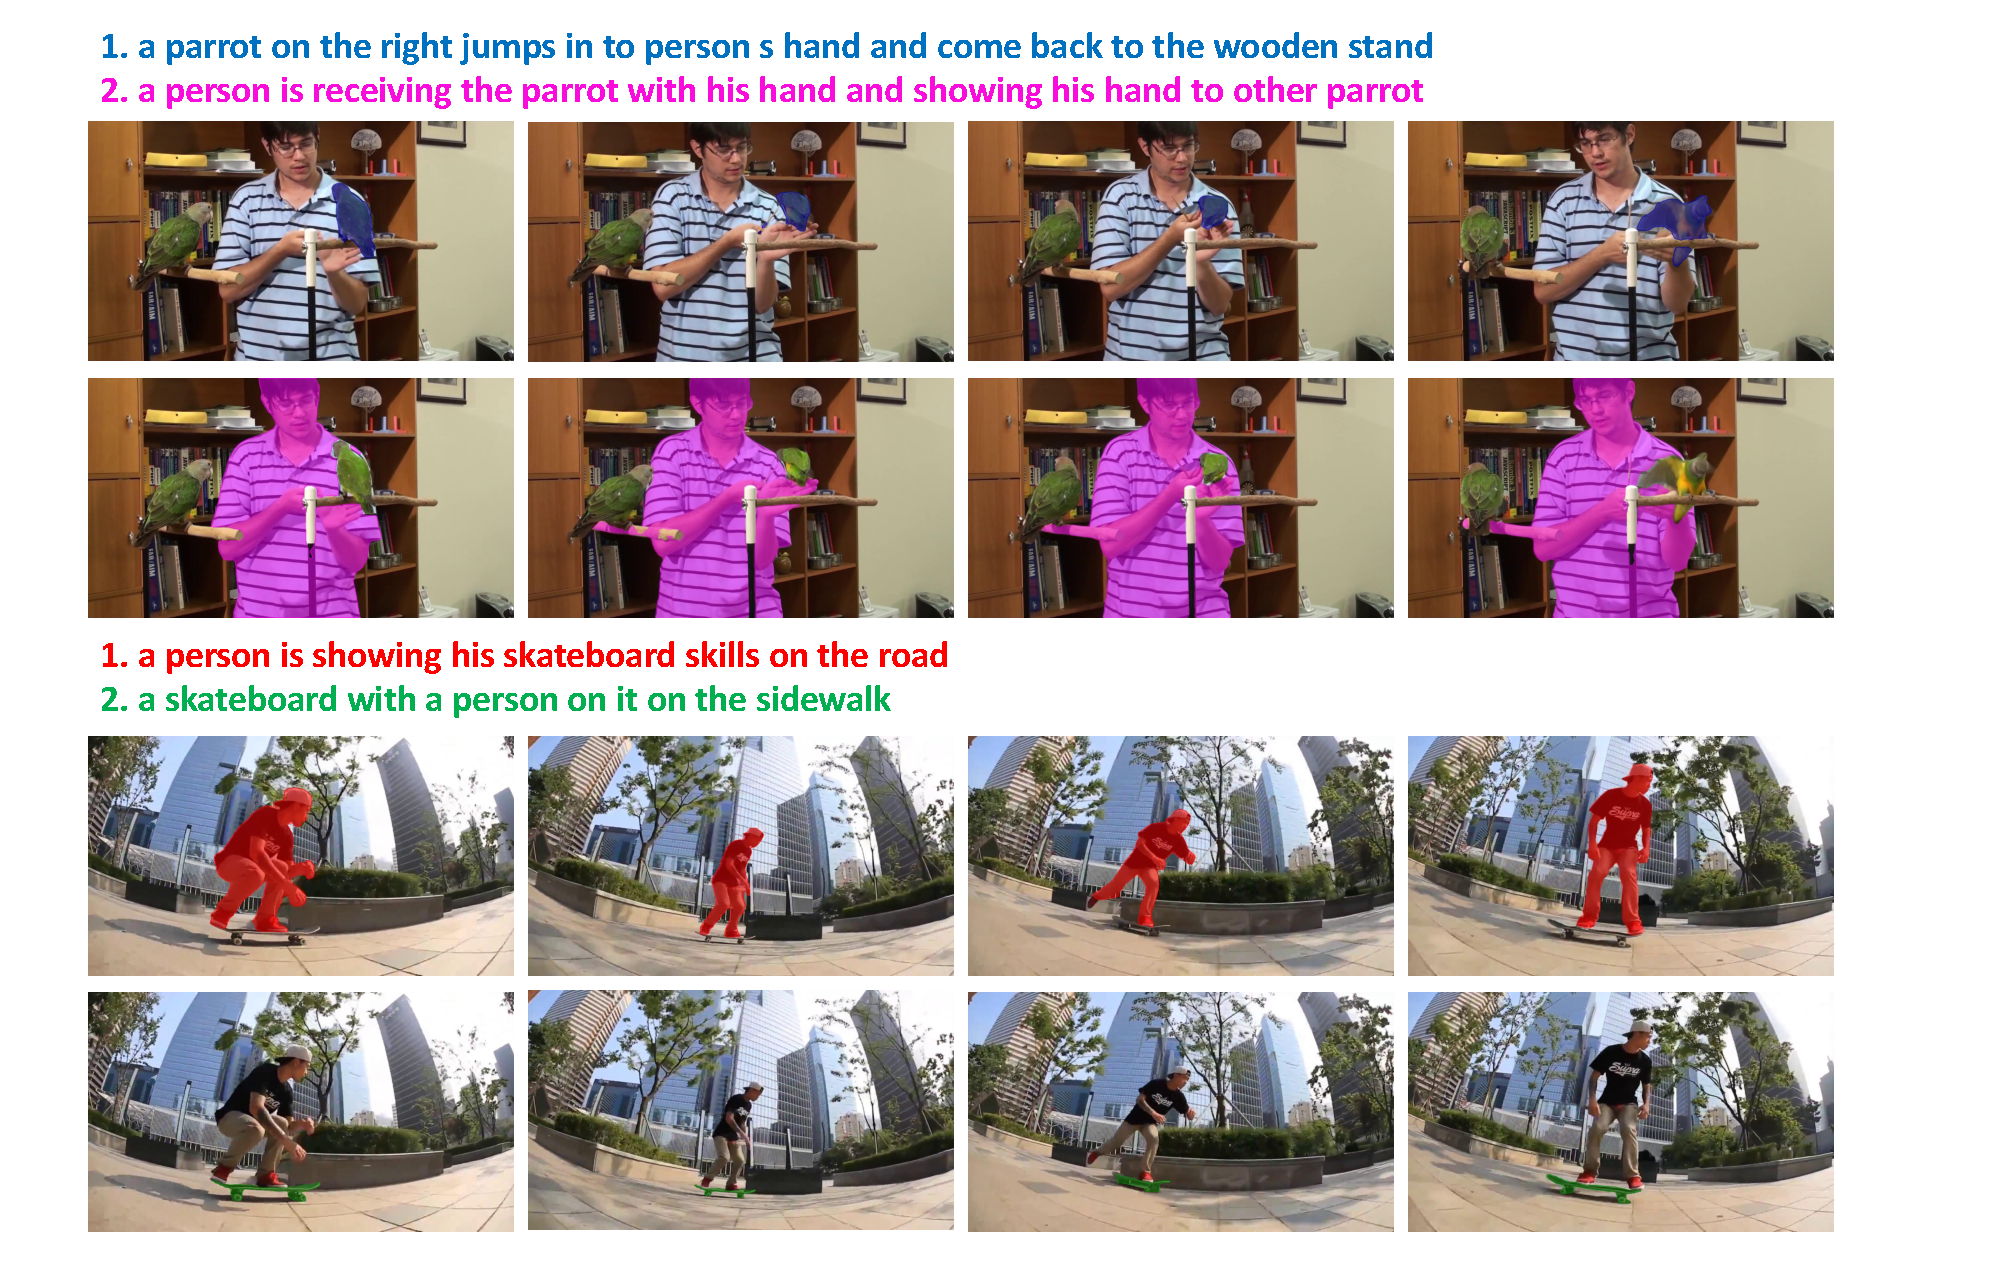
\includegraphics[width=\textwidth]{content/resources/images/referring_segmentation/QualitativeResults.pdf}
    \caption{\textbf{Qualitative results} on Refer-YouTube-VOS dataset. Each referring expression and the corresponding referred object are highlighted in the same color.}
    \label{fig:refyoutube_qualitative}
\end{figure}

Figure \ref{fig:refyoutube_qualitative} shows the qualitative results of our proposed model on the Refer-YouTube-VOS dataset. Each referring expression and the corresponding object are highlighted in the same color. The first two rows of images are about a video about a man standing with two parrots. The first expression \textit{"a parrot on the right jumps into person's hand and come back to the wooden stand"} describes the parrot on the right (blue color), and our model can segment almost perfectly. In the same video, the expression "a person is receiving the parrot with his hand and showing his hand to other parrot" refers to the man behind two parrots (pink color). Our model segments the person accurately except for the wooden stick nearby. 



\begin{figure*}[t]
    \centering
    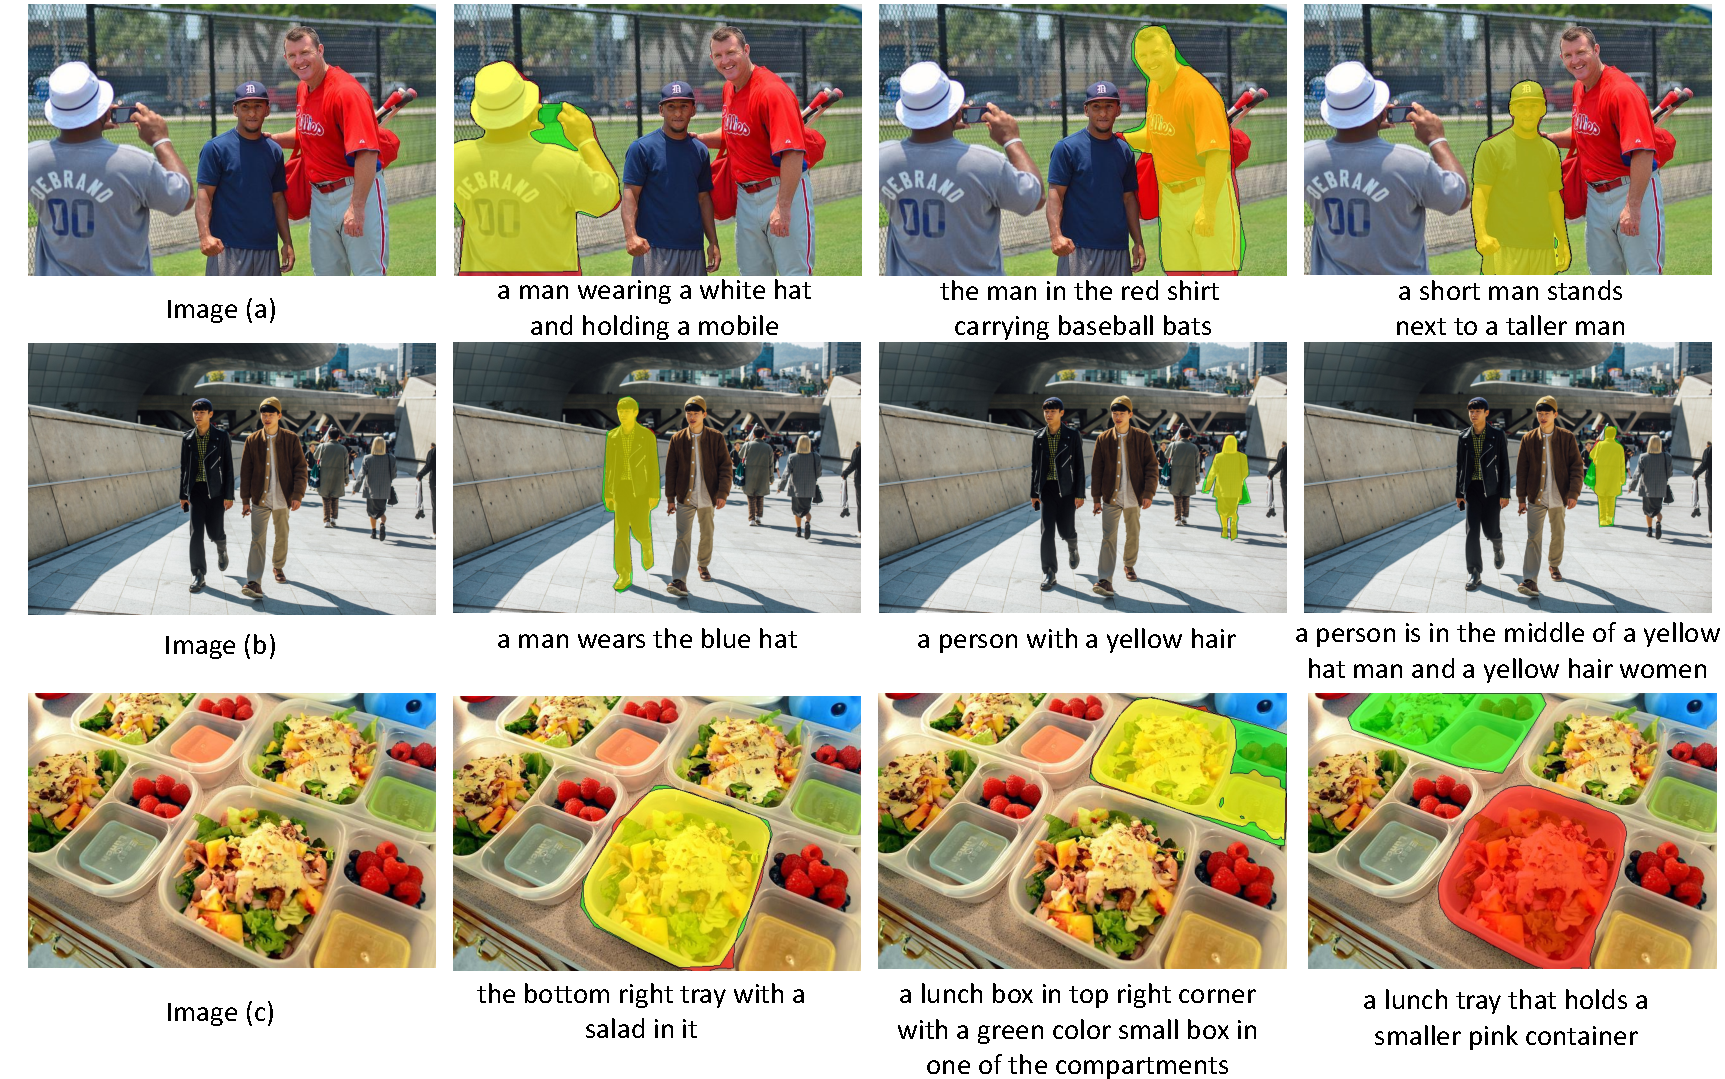
\includegraphics[width=0.8\textwidth]{content/resources/images/referring_segmentation/Visualization_New.pdf}
    \caption{The visualization of referring image segmentation results. From left to right: the input image, our overlaid results with the corresponding expressions. Overlaid color legend: green and red indicate the groundtruth and our segmentation results, respectively; while yellow highlights the intersection between the ground truth and our results.  }
    \label{fig:visualization}
\end{figure*}

We visualize the referring image segmentation results from our method in Figure \ref{fig:visualization}. To illustrate the impressive ability of our method, we show the predicting results of some examples with different expressions. Image (a) shows that our method can handle the expression containing the color information. The last image in the first row even demonstrates the capability to segment objects with attributes about the relative height, i.e., short, tall. In (b), we can see that our network can understand the color, i.e., blue, yellow and related stuff, i.e., hat, hair, and also identifies the referred person who locates in the middle of the two described objects. In (c), VLFormer correctly identifies the correct objects in the first two expressions. However, the third expression regarding the ``smaller pink container'' is confusing since there is no obvious pink container in the image. Therefore, VLFormer picks a pinkish object. This incorrect segmentation illustrates the failure case in our proposed work.

% Figure \ref{fig:visualization} also shows our model's ability to segment the referred object through a variety different target expressions. 

% \begin{figure}[ht]
%     \centering
%     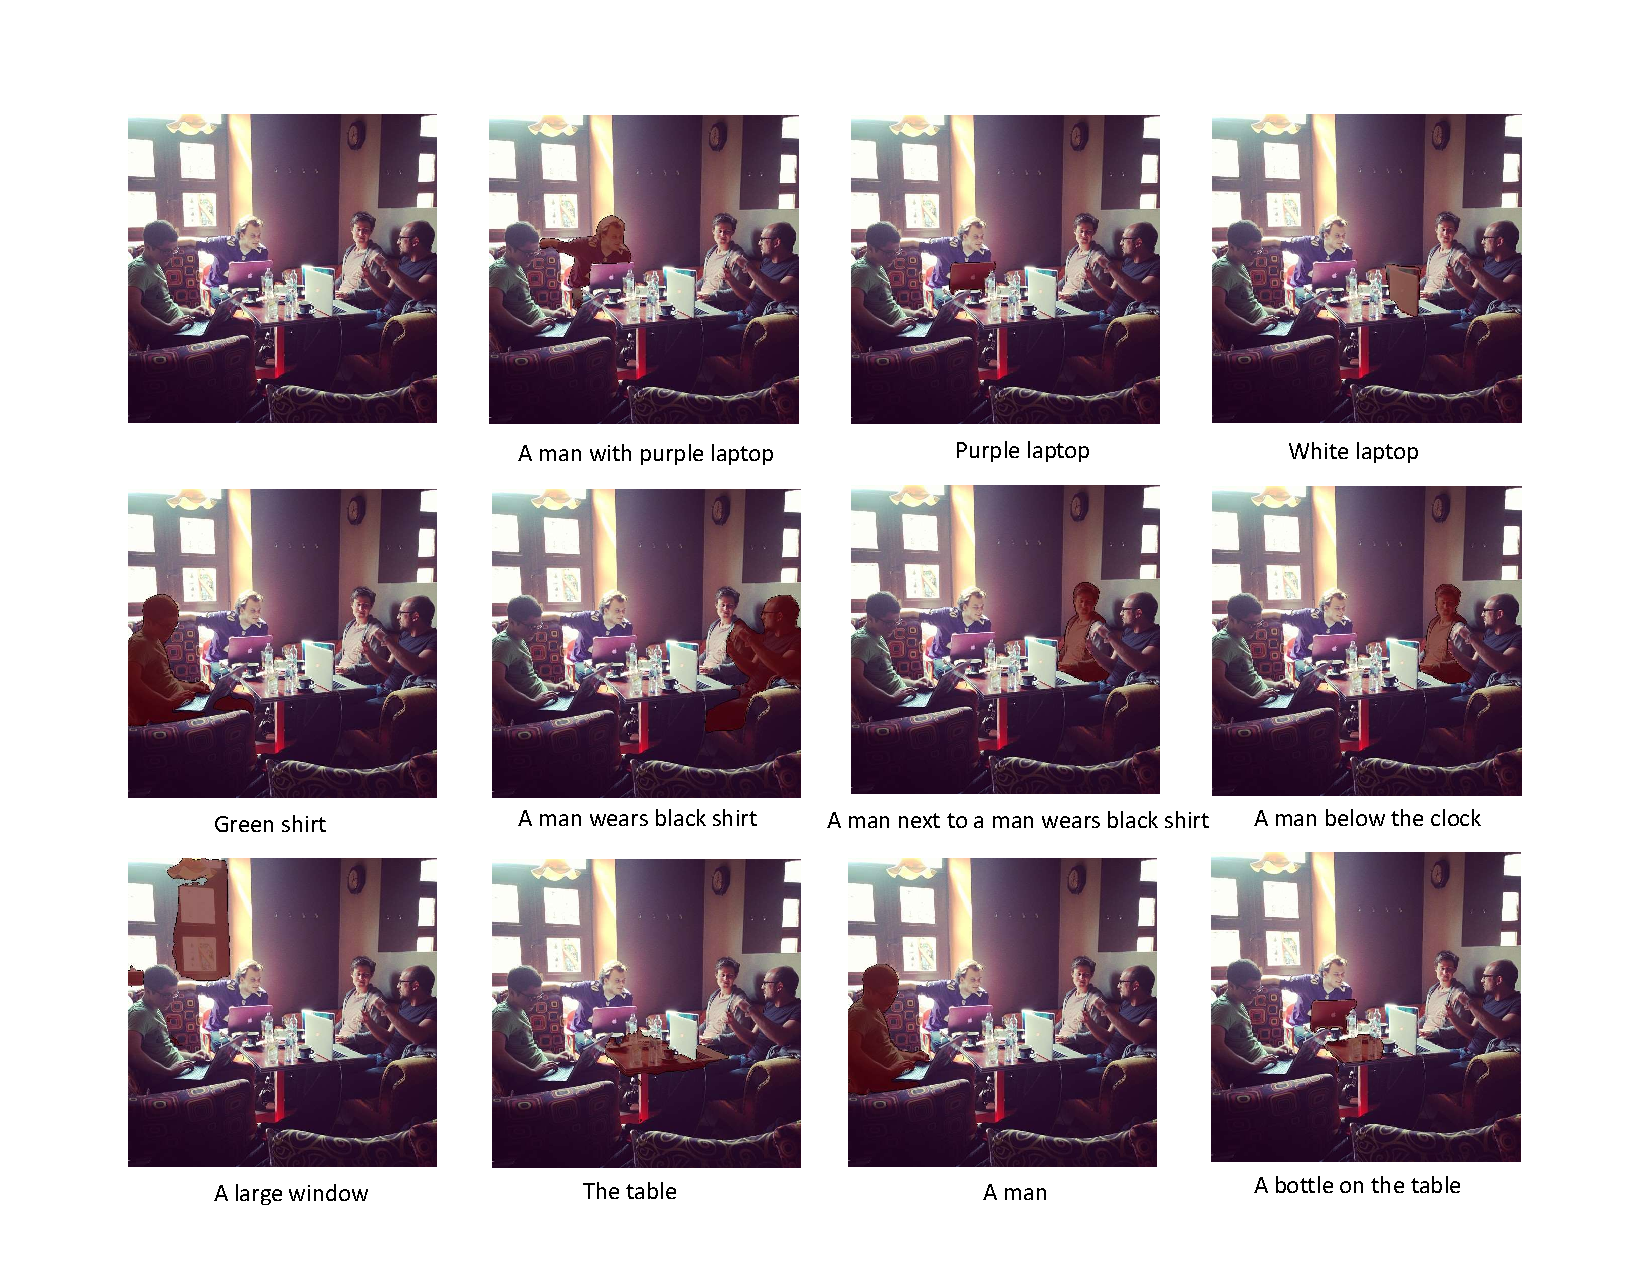
\includegraphics[width=\textwidth]{content/resources/images/referring_segmentation/Visualization.pdf}
%     \caption{Visualization. Diversity of referring expressions for an image. }
%     \label{fig:visualization}
% \end{figure}

\section{Apply Referring Expression Segmentation into Retrieval System}
The interactive retrieval system allows users to search for relevant images by inputting a language query. The system then retrieves matching images from the database, which usually contains the objects or concepts referred to in the query. This retrieval system and referring expression segmentation task uses both the text query and images as input. This shared input helps us to leverage the referring segmentation in our retrieval system, providing explainability and reliability in the retrieval results.

In our retrieval system, when a query is sent, the system responds with a rank-list of relevant images almost instantly. However, our referring expression segmentation module is not too fast (18 FPS). Therefore, to enhance the user experience, we leverage the text query to precisely point out the target object or concept referred to in the images that belong to the rank-list only.

Figure \ref{fig:res_retrieval_system} illustrates the using referring segmentation in our retrieval system for the explainability. It can be seen that the results are promising. With the query "a man next to the whiteboard", our system retrieves several images containing a man and a whiteboard next to him.
In most of the images, we successfully segment the person who stands right next to a whiteboard. In other cases, which contain no people in the images, our module even points out the whiteboard instead of a human, which is a reasonable replacement.


\begin{figure}[!t]
    \centering
    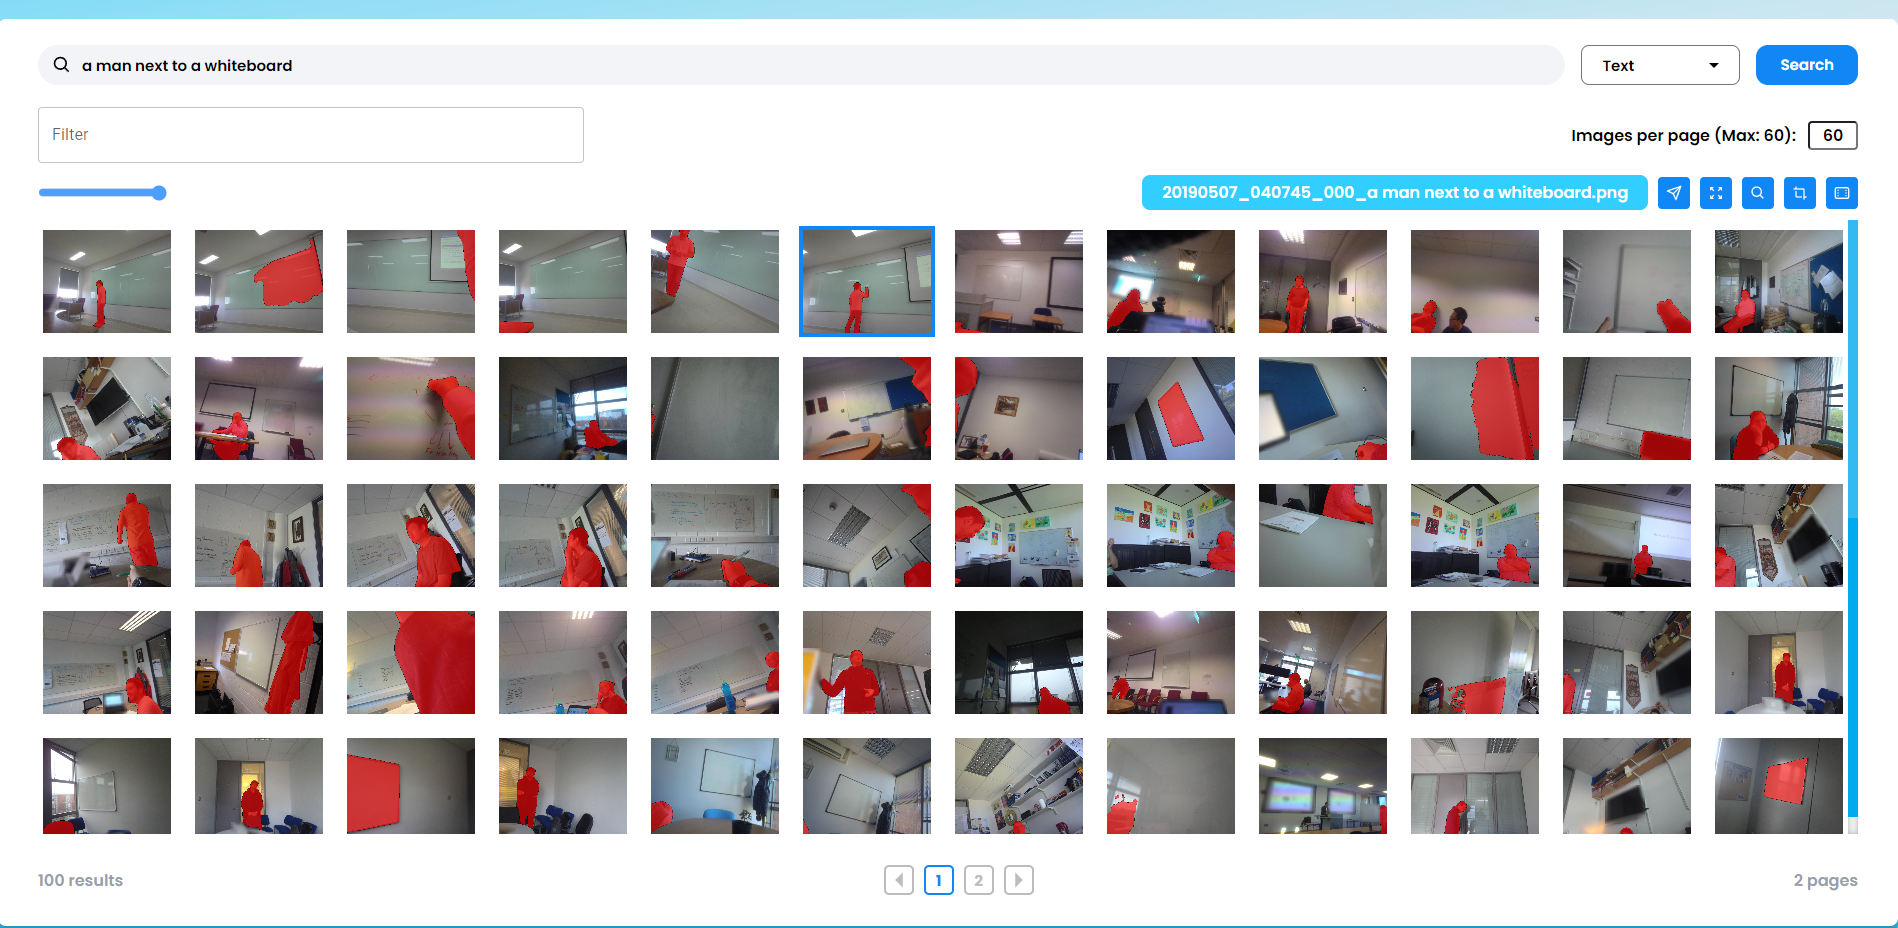
\includegraphics[width=0.8\linewidth]{content/resources/images/referring_segmentation/ReferringSegmentationInRetrievalSystem.png}
    \caption{An example of using referring expression segmentation in our retrieval system for the explainable retrieval results. The referred object is highlighted in the retrieval results in red color.}
    \label{fig:res_retrieval_system}
\end{figure}

